% !TeX root = main.tex
\documentclass[11pt,a4paper,UTF8]{ctexart}
\usepackage{quicklatex} % 引入自定义样式
\usepackage[toc,page]{appendix}

\title{端侧文生多模态大模型文献综述}
\author{邱梓豪}
\date{\today}

\begin{document}



\maketitle
\tableofcontents
\newpage

\section{前言}

在本篇文献综述中,我们对端侧文生图模型的核心技术进展进行了系统梳理与评述。全文结构分为四个递进部分,涵盖理论基础、算法创新、模型实现与端侧优化等关键环节,为研究者提供完整的技术图谱。

第一部分聚焦于扩散模型的数学理论基础。我们将详细介绍扩散模型的三大核心理论框架:去噪扩散概率模型、基于分数的生成模型以及随机微分方程方法。在此基础上,系统推导条件生成场景下的数学表达,深入阐释文本到图像生成的概率建模机制,为后续算法与实际应用奠定坚实的理论基础。

第二部分系统梳理了扩散模型的关键算法创新。重点论述以下四方面的最新进展:(1)少步数扩散模型范式;(2)高效采样算法;(3)似然估计优化方法;(4)流形空间上的扩散建模。这些算法改进大大提升了模型的生成质量、效率和实际可用性,其中许多已成为当前主流方法的标准配置。

第三部分深入探讨文生图模型在实际应用中的关键实现要素。具体包括模型架构设计、训练数据构建以及主流扩散模型的评测基准,从而为扩散模型的高效训练与评估提供系统指导,促进其落地部署和广泛应用。

第四部分则专门聚焦端侧部署所面临的技术挑战。针对移动设备等边缘计算场景下的计算资源受限问题,我们将详述:(1)参数量化与稀疏化技术;(2)轻量级网络结构设计;(3)基于蒸馏的压缩方法——包括参数蒸馏与步数蒸馏;(4)底层计算优化策略。通过这些技术手段的协同应用,推动高效文生图模型在端侧的落地与规模化应用。

综上,本综述旨在全面梳理端侧文生图模型从理论到实践的技术链条,为相关领域研究与工程实现提供系统参考,助力高效生成模型在移动端等实际场景中的深度应用。

\newpage

\section{扩散模型数学基础}

【这里可以用一张表或图进行总结】

本节系统阐述扩散模型的核心理论基础,涵盖三大主流范式:去噪扩散概率模型(Denoising Diffusion Probabilistic Model,DDPM)\cite{sohldickstein2015diffusion,ho2020denoising}、基于分数的生成模型(Score-based Generative Model,SGM)\cite{song2019generative,song2020improved},以及基于随机微分方程的分数模型(Score SDE)\cite{song2020score,karras2022elucidating}。这三类方法本质上都遵循“先扰动、后生成”的思想框架:首先以逐步注入噪声的方式设计前向扩散过程,将结构化数据渐进变为噪声分布;再以反向去噪重建实现新样本生成。本节将依次梳理各类扩散模型的前向及反向机制,揭示模型之间的内在联系,最后介绍条件生成场景下的扩散模型数学表达形式。

我们首先统一扩散模型中常用记号。设离散时间步为$t\in\{0,1,\cdots,T\}$,连续时间变量为$t\in[0,T]$。记原始数据为$\x_0\in\R^d$,满足$\x_0\sim q(\x_0)$。扩散模型通过向原始数据中不断加入高斯噪声构造一条数据轨迹$\{\x_0,\x_1,\cdots,\x_T\}$,最终使$\x_T$趋近于标准高斯分布。噪声注入强度由调度系数$\beta_t$(离散场景)或时变函数$\beta(t)dt$(连续场景)进行控制。


\subsection{去噪扩散概率模型 (DDPM)}

去噪扩散概率模型(Denoising Diffusion Probabilistic Model, DDPM)的核心框架基于两条相互关联的马尔可夫链:前向扩散链通过逐步添加噪声将原始数据分布扰动为简单的已知先验分布(如标准高斯分布),其中噪声调度可采用预设的固定策略;而反向生成链则通过可学习的参数化转移核(transition kernel)实现噪声到数据的渐进式重建,该转移核一般由深度神经网络进行参数化建模,其本质是通过训练来逼近前向扩散过程的逆过程。在生成阶段,模型首先从先验分布中抽取随机噪声向量,随后通过反向链执行多步\emph{祖先采样}(ancestral sampling)\cite{koller2009probabilistic}——即每一步的采样都严格依赖于前一步的隐变量状态,这种序列化采样机制最终将噪声逐步转化为符合目标数据分布的新样本。

\subsubsection{DDPM的前向与反向过程}

下面我们给出去噪扩散概率模型(DDPM)前向与反向过程的数学表述。设原始数据分布为$\x_0\sim q(\x_0)$,前向扩散过程定义为一个参数化的马尔可夫链,它通过转移核$q(\x_t|\x_{t-1})$生成隐变量序列(或称数据轨迹)$\{\x_0,\x_1,\cdots,\x_T\}$。根据马尔可夫性质,该过程的联合分布可分解为:
\begin{equation*}
    q(\x_1,\cdots,\x_T|\x_0)=\prod_{t=1}^T q(\x_t|\x_{t-1}).
\end{equation*}

在标准DDPM框架中,前向转移核$q(\x_t|\x_{t-1})$采用高斯扰动形式:
\begin{equation}
    q(\x_t|\x_{t-1}) =\N(\x_t;\sqrt{1-\beta_t}\x_{t-1},\beta_t\mathbf{I}),
\label{ddpm:forward_process}
\end{equation}
其中$\beta_t\in(0,1)$是预先设定的噪声调度系数,$\mathbf{I}$是单位对角矩阵。正如Sohl-Dickstein等人\cite{sohldickstein2015diffusion}所述,使用上面设计的好处在于我们可以方便地获得某时间步$t\in\{0,1,\cdots,T\}$的数据$\x_t$的边缘分布。具体地,给定$\x_0$时$\x_t$的条件分布如下:
\begin{equation}
    q(\x_t|\x_0)=\N(\x_t;\sqrt{\bar{\alpha}_t}\x_0,(1-\bar{\alpha}_t)\mathbf{I}),
\label{ddpm:bar_alpha}
\end{equation}
其中$\alpha_t:=1-\beta_t$,$\bar{\alpha}_t:=\prod_{s=0}^t\alpha_s$。可以看出,上式实际上允许我们通过重参数化技巧(reparameterization trick)进行高效采样,即对于标准高斯噪声$\epsilon\in\N(0,\mathbf{I})$,$\x_t$的采样可表示为:
\begin{equation*}
    \x_t=\sqrt{\bar{\alpha}_t}\x_0 + (1-\bar{\alpha}_t)\epsilon.
\end{equation*}
值得注意的是,当$T$足够大时,$\bar{\alpha}_T\approx 0$,使得边缘分布$q(\x_T)=\int q(\x_T|\x_0)q(\x_0)d\x_0$渐进收敛于标准高斯分布$\N(\mathbf{0},\mathbf{I})$,从而满足前向过程将数据完全扩散为噪声的设计目标。

从直观上看,前向扩散过程通过逐步注入噪声使数据结构性信息持续衰减,最终退化为无结构噪声。为了实现数据生成,DDPM首先从先验分布$p(\x_T)=\N(\x_T;\mathbf{0},\mathbf{I})$采样纯噪声(该设定的合理性源于前向过程保证$q(\x_T) \approx \mathcal{N}(\x_T; \mathbf{0}, \mathbf{I})$),随后通过可学习的反向马尔可夫链逐步去噪重构数据。该反向链的核心是参数化转移核:
\begin{equation}
    p_{\theta}(\x_{t-1}|\x_t) = \N(\x_{t-1};\mu_{\theta}(\x_t,t),\Sigma_{\theta}(x_t,t)),
\label{ddpm:reverse_gaussian}
\end{equation}
其中$\theta$表示模型参数,高斯均值$\mu_{\theta}(\x_t,t)$和方差$\Sigma_{\theta}(x_t,t))$函数由深度神经网络进行参数化,并以带噪声的数据样本$\x_t$和时间$t$为输入。假设我们可以充分学习$p_{\theta}(\x_{t-1}|\x_t)$,那么便可以通过先从$p(\x_T)=\N(\x_T;\mathbf{0},\mathbf{I})$采样$\x_T$,再迭代式地调用$p_{\theta}(\x_{t-1}|\x_t)$(直到$t=1$)来生成样本$\x_0$。完整的生成流程可表述为:
\begin{equation*}
\x_T \sim p(\x_T) \rightarrow \x_{T-1} \sim p_{\theta}(\x_{T-1}|\x_T) \rightarrow \cdots \rightarrow \x_0 \sim p_{\theta}(\x_0|\x_1).
\end{equation*}
在下一节,我们将推导DDPM的目标函数,并展示如何通过数学推导和特定的参数化设计得到方便计算优化的$\mu_{\theta}(\x_t,t)$和$\Sigma_{\theta}(x_t,t))$形式。


\subsubsection{DDPM的训练与推理}

DDPM的核心训练目标在于学习反向条件分布$p_{\theta}(\x_{t-1}|\x_t)$,该目标通过变分推断框架实现\cite{sohldickstein2015diffusion}。具体而言,基于前向扩散过程建立的马尔可夫链特性,模型通过最大化观测数据对数似然$\log p_{\theta}(\x_0)$的变分下界(ELBO)进行优化。这一理论框架将自然地引出了均值函数$\mu_{\theta}(\x_t,t)$和方差函数$\Sigma_{\theta}(\x_t,t)$的构造方法,并可由此进一步简化目标函数,最终转化为可高效优化的噪声预测任务\cite{ho2020denoising}。

给定数据样本$\x_0\sim q(\x_0)$,反向生成$\x_0$的对数似然为$\log p_{\theta}(\x_0)$的ELBO形式可由Jensen不等式及前向/反向过程的马尔可夫性质推导而来(推导详细见附录\ref{app:ddpm_elbo}):
\begin{equation}
\log p_{\theta}(\x_0) \geq \E_q[\log p_{\theta}(\x_0|\x_1)]  - \sum_{t=2}^{T} \mathbb{E}q \left[ \mathrm{KL} (q(\x_{t-1}|\x_t,\x_0)||p_\theta(\x_{t-1}|\x_t)) \right] + \text{const},
\label{eq:ddpm-elbo}
\end{equation}
其中$q(\x_{t-1}|\x_t,\x_0)$为前向过程的“后验”分布,$p_\theta(\x_{t-1}|\x_t)$为可学习的反向分布,KL散度量化了模型在反向还原过程中对数据分布的逼近程度,$\text{const}$项中不包含可学习的参数。于是我们可以定义\emph{变分下界损失}$\mathcal{L}_{\text{VLB}}$如下:
\begin{equation}
\mathcal{L}_{\text{VLB}} := -\E_q [\log p_{\theta}(\x_0|\x_1)] +  \Sigma_{t=2}^T \text{KL}(q(\x_{t-1}|\x_t,\x_0) \| p_{\theta}(\x_{t-1}|\x_t)),
\label{ddpm:loss_vlb}
\end{equation}
显然,最小化$\mathcal{L}_{\text{VLB}}$即是最大化(\ref{eq:ddpm-elbo})中的变分下界,等价于最大化扩散模型生成数据的似然。

$q(\x_{t-1}|\x_t,\x_0)$经过推导(详见附录\ref{app:ddpm_forward_posterior_distribution}),可以证明其具有如下高斯分布形式:
\begin{align}
\begin{split}
    q(\x_{t-1}|\x_t,\x_0) &= \N(\x_{t-1}|\mu_q(\x_t,\x_0),\Sigma_q(t)),\\
    \mu_q(\x_t,\x_0) &= \frac{(1-\bar{\alpha}_{t-1})\sqrt{\alpha_t}}{1-\bar{\alpha}_t}\x_t + \frac{(1-\alpha_t)\sqrt{\bar{\alpha}_{t-1}}}{1-\bar{\alpha}_t}\x_0 \\
    \Sigma_q(t) &= \frac{(1-\alpha_t)(1-\bar{\alpha}_{t-1})}{1-\bar{\alpha}_t}\mathbf{I}  \stackrel{\text{def}}{=} \sigma_q^2(t)\mathbf{I},
\end{split}
\label{eq:reverse-posterior-main}
\end{align}
其中$\bar{\alpha}_t=\Pi_{i=1}^t \alpha_i$。为便于解析计算及模型优化,反向分布$p_{\theta}(\x_0|\x_1)$也采用高斯分布建模,即
\begin{equation*}
    p_{\theta}(\x_0|\x_1)=\N(\x_{t-1}| \mu_{\theta}(\x_t,t), \sigma_q^2(t)\mathbf{I}),
\end{equation*}
其中,均值参数$\mu_\theta(\x_t,t)$由神经网络$\mu_{\theta}(\x_t,t)$预测,方差项通常与前向过程一致,即$\sigma_q^2(t)\mathbf{I}$。于是(\ref{eq:ddpm-elbo})中的KL散度可简化为:
\begin{align}
\begin{split}
    \text{KL}\left(q(\x_{t-1}|\x_t,\x_0) \| p_{\theta}(\x_{t-1}|\x_t)\right) &= \text{KL} \left(\N(\x_{t-1}|\mu_q(\x_t,\x_0),\sigma_q^2(t)\mathbf{I}) \| \N(\x_{t-1}| \mu_{\theta}(\x_t,t), \sigma_q^2(t)\mathbf{I})\right) \\
    &= \frac{1}{2\sigma_q^2(t)} \| \mu_q(\x_t,\x_0) - \mu_{\theta}(\x_t,t) \|^2,
\label{ddpm:elbo_simp_1}
\end{split}
\end{align}
上面利用了两方差相同的高斯分布间的KL散度可简化为其均值向量间的平方欧式距离这一点。

此外,对于变分下界(\ref{eq:ddpm-elbo})中的$\log p_{\theta}(\x_0|\x_1)$可以进行如下简化:
\begin{align}
\begin{split}
&\log p_{\theta}(\x_0|\x_1) = \log \N(\x_0| \mu_{\theta}(\x_1,1),\sigma_q^2(1)\mathbf{I}) \\
&= \log \left( \frac{1}{\left(\sqrt{2\pi\sigma_q^2(1)} \right)^d} \right)\exp \left\{-\frac{\|\x_0 -\mu_{\theta}(\x_1,1) \|^2}{2\sigma_q^2(1)} \right\} \\
&= -\frac{\|\x_0 -\mu_{\theta}(\x_1,1) \|^2}{2\sigma_q^2(1)} -\frac{d}{2}\log (2\pi\sigma_q^2(1)),
\label{ddpm:elbo_simp_2}
\end{split}
\end{align}
可以看出(\ref{ddpm:elbo_simp_1})和(\ref{ddpm:elbo_simp_2})从优化目标上实际上是统一的,都是\emph{最小化前向过程产生的数据轨迹和对应的反向过程生成的数据轨迹的欧式距离}。

下面,我们再对$\mu_q(\x_t,\x_0)$的具体形式进行分析,并由此设计$\mu_{\theta}(\x_t,t)$的计算方式,最后完成DDPM目标函数的推导。我们由$q(\x_t|\x_0)$的表达式可知:
\begin{equation*}
    \x_t =\sqrt{\bar{\alpha}_t}\x_0 + \sqrt{1-\bar{\alpha}_t}\epsilon \Rightarrow  \x_0 =\frac{\x_t - \sqrt{1-\bar{\alpha}_t}\epsilon}{\sqrt{\bar{\alpha}_t}}.
\end{equation*}
随后我们将上式代入(\ref{eq:reverse-posterior-main})中$\mu_q(\x_t,\x_0)$的表达式,可以得到:
\begin{align}
\begin{split}
    \mu_q(\x_t,\x_0) &= \frac{(1-\bar{\alpha}_{t-1})\sqrt{\alpha_t}\x_t +(1-\alpha_t)\sqrt{\bar{\alpha}_{t-1}}\x_0 }{1-\bar{\alpha}_t} \\
    &= \frac{(1-\bar{\alpha}_{t-1})\sqrt{\alpha_t}\x_t +(1-\alpha_t)\sqrt{\bar{\alpha}_{t-1}}\frac{\x_t - \sqrt{1-\bar{\alpha}_t}\epsilon}{\sqrt{\bar{\alpha}_t}} }{1-\bar{\alpha}_t}\\
    &= \frac{1}{\sqrt{\alpha_t}}\x_t - \frac{1-\alpha_t}{\sqrt{1-\bar{\alpha}_t}\sqrt{\alpha_t}}\epsilon,
\end{split}
\label{ddpm:mu_q}
\end{align}
上式实际上将$\mu_q(\x_t,\x_0)$由关于$\x_0$的函数转化成关于高斯噪声$\epsilon$的函数。受此启发,下面我们将设计一个更合适的$\mu_{\theta}(\x_t,t)$的形式,使之适配$\mu_q(\x_t,\x_0)$的表达式,具体地,我们进行如下设计:
\begin{equation}
\mu_{\theta}(\x_t,t)=\frac{1}{\sqrt{\alpha_t}}\x_t - \frac{1-\alpha_t}{\sqrt{1-\bar{\alpha}_t}\sqrt{\alpha_t}}\epsilon_{\theta}(\x_t,t),
\label{ddpm:mu_theta}
\end{equation}
值得注意的是,我们此时让模型预测第$t$步中向$\x_t$中加入的噪声,即$\epsilon_{\theta}(\x_t,t)$。

最后,我们将(\ref{ddpm:elbo_simp_1})、(\ref{ddpm:elbo_simp_2})、(\ref{ddpm:mu_q})和(\ref{ddpm:mu_theta})代入(\ref{eq:ddpm-elbo}),并结合(\ref{ddpm:loss_vlb})的定义,可得:
\begin{equation}
\mathcal{L}_{\text{VLB}} = -\sum_{t=1}^T \E_q \left[\frac{1}{2\sigma_q^2(t)}\frac{(1-\alpha_t)^2}{(1-\bar{\alpha}_t)\alpha_t}\|\epsilon_{\theta}(\x_t,t)-\epsilon \|^2 \right],
\label{ddpm:loss_vlb_denoise}
\end{equation}
于是我们最终得到了DDPM的目标函数,它实际上是一个监督学习型的目标函数,即训练扩散模型的输出,即$\epsilon(\x_t,t)$,来预测前向过程中每一步加入的噪声$\epsilon$。注意,实际上加入的噪声是$\epsilon$乘上某系数,但我们设计扩散模型反向过程中也让$\epsilon(\x_t,t)$乘上此系数,所以在(\ref{ddpm:loss_vlb_denoise})中该系数可以被提取出来,形成系数$\frac{1}{2\sigma_q^2(t)}\frac{(1-\alpha_t)^2}{(1-\bar{\alpha}_t)\alpha_t}$。

最后我们介绍扩散模型的生成过程。在训练结束后,我们可以获得神经网络$\epsilon_{\theta}(\x_t,t)$。生成新样本时,我们先采样一个高斯白噪声$\x_T\sim\N(\mathbf{0},\mathbf{I})$,随后便可以利用(\ref{ddpm:mu_q})中建立的$\x_{t-1}$与$\x_t$的关系以及(\ref{ddpm:mu_theta})中$\mu_\theta$的定义,迭代式地生成$\x_{T-1},\cdots,\x_0$,具体的计算方式为:
\begin{equation*}
    \x_{t-1} = \frac{1}{\sqrt{\alpha_t}}\left(\x_t -\frac{1-\alpha_t}{\sqrt{1-\bar{\alpha}_t}} \epsilon(\x_t,t) \right) + \sigma_q(t)\z,\quad \z\sim\N(\mathbf{0},\mathbf{I}).
\end{equation*}

\subsection{基于分数的生成模型 (SGM)}

本节将系统阐述基于分数的生成模型(Score-based Generative Models, SGM)的理论框架。首先,我们将从Stein分数函数(简称分数函数)的基本概念与数学定义入手,建立理论基础;随后,我们深入探讨分数函数匹配(Score Matching)这一主流学习范式的原理与实现方法;最后,重点介绍当前SGM领域的前沿方法——噪声条件分数网络(Noise Conditional Score Network, NCSN)\cite{song2020score}。

\subsubsection{Stein分数函数}

基于分数的生成模型的核心在于利用Stein分数函数(简称分数函数)\cite{Hyvrinen2005EstimationON}这一关键工具。对于给定的样本概率密度函数$p(\x)$,其Stein分数函数定义为对数概率密度的梯度场:
\begin{equation*}
    \s_\theta(\x) := \nabla_{\x}\log p(\x).
\end{equation*}
需要特别强调的是,此定义与统计学中常见的Fisher分数$\nabla_\theta \log p_{\theta}(\x)$存在本质区别:Stein分数函数关注的是\emph{样本空间}上的梯度变化,而非模型参数空间$\theta$的梯度信息。这一向量场揭示了数据分布的内在几何特征,其方向指示了使数据出现概率增加最快的路径。

当我们获得分数函数$\nabla_{\x}\log p(\x)$后,便可以通过朗之万动力学(Langevin dynamics)来从目标分布$p(\x)$中采样。具体地,给定步长$\alpha>0$以及一个初始值$\tilde{\x}_0\sim\pi(\x)$($\pi(\x)$为任意先验分布),采样过程通过以下迭代公式完成:
\begin{equation*}
    \tilde{\x}_t = \tilde{\x}_{t-1} + \frac{\alpha}{2} \nabla_{\x}\log p(\tilde{\x}_{t-1}) + \sqrt{\alpha}\epsilon_t,\quad \epsilon_t\sim\N(\mathbf{0},\mathbf{I}).
\end{equation*}

当某些正则性条件被满足时,若$\alpha\rightarrow 0$且$T\rightarrow \infty$,\cite{max2011bayesian}的理论分析说明$\tilde{\x}_T$的分布将精确收敛于$p(\x)$。当$\alpha> 0$且$T< \infty$时上面的公式存在一些误差,需要用Metropolis-Hastings更新来修正,但在实践中通常可以忽略这种修正\cite{du2019implicit,nijkamp2019anatomy}。本文的后续分析将基于这一合理的工程假设展开。

上述理论框架揭示了基于分数的生成模型的核心优势:通过建立分数函数估计与朗之万动力学采样之间的数学联系,实现了从数据分布中直接采样的可能性。这种方法的有效性主要依赖于两个关键因素——对目标分布分数函数的准确估计,以及朗之万动力学过程的合理配置。下面我们将围绕这两个核心要素展开深入探讨。

\subsubsection{分数函数匹配}

在分数函数学习方法的演进过程中,研究者们提出了多种技术路线。一种方法称为显式分数函数匹配(Explicit Score Matching,ESM)\cite{vincent2011connection}。假设我们有一个包含$M$个样本的数据集$\X=\{\x^{(1)},\cdots,\x^{(M)}\}$,那么我们可以通过\emph{核密度估计}来近似真实数据分布$p(\x)$:
\begin{equation*}
    q_h(\x)=\frac{1}{M}\sum_{m=1}^M \frac{1}{h} K\left(\frac{\x-\x^{(m)}}{h} \right),
\end{equation*}
其中$K(\cdot)$是核函数,$h$是核函数的超参数。随后显式分数函数匹配基于$q_h(\x)$来学习分数函数$\s_\theta(\x)$,目标函数如下:
\begin{equation*}
    \mathcal{L}_{\text{ESM}}:=\frac{1}{2}\E_{p(\x)} \|\s_\theta(\x)-\nabla_{\x}\log p(\x) \|^2 \approx \frac{1}{2}\E_{q_h(\x)} \| s_\theta(\x)-\nabla_{\x}\log q_h(\x)\|^2.
\end{equation*}
该方法的主要问题在于核密度是非参数化的、它对真实分布的近似能力很有限,尤其是当样本数量有限或数据处于高维空间时,核密度估计的效果会较差。

为了避免近似真实数据分布,\cite{Hyvrinen2005EstimationON}提出了隐式分数函数匹配(Implicit Score Matching,ISM),其目标函数为:
\begin{equation*}
    \mathcal{L}_{\text{ISM}}:=\E_{p(\x)} \left[\text{Tr}(\nabla_{\x} \s_\theta (\x)) + \frac{1}{2}\|\s_\theta (\x) \|^2 \right],
\end{equation*}
其中$\nabla_{\x} \s_\theta (\x)$表示$\s_\theta (\x)$的Jacobian。尽管该方法避免了直接近似真实数据分布$p(\x)$,但\cite{song2019generative}指出该目标函数的迹函数难以计算,导致该方法缺乏可扩展性。

现在最流行的分数函数学习方法是基于去噪分数函数匹配(Denoising Score Matching,DSM)\cite{vincent2011connection}。给定一个样本$\x_0$,该方法使用一个预定义的噪声分布$q_\sigma(\x^\prime|\x)$对其进行扰动得到带噪声数据,其分布为$q_\sigma(\x^\prime):=\int q_\sigma(\x^\prime|\x)p(\x)d\x$。DSM的核心思想是使用分数函数匹配来估计\emph{该带噪声数据分布$q_\sigma(\x^\prime)$的分数函数},优化目标如下:
\begin{equation}
\E_{q_\sigma(\x^\prime|\x)p(\x)} \left[\frac{1}{2}\| \s_{\theta}(\x^\prime) - \nabla_{\x^\prime}\log q(\x^\prime|\x) \|^2 \right].
\label{sgm:dsm}
\end{equation}
\cite{vincent2011connection}的结论显示最小化以上目标函数得到的最优分数函数(记为$\s_{\theta^*}(\x)$)\emph{几乎必然满足}$\s_{\theta^*}(\x)=\nabla_\x\log q_\sigma(\x)$。值得注意的是,只有当噪声足够小时,才有$q_\sigma(\x)\approx p(\x)$成立。

为了高效地计算(\ref{sgm:dsm}),一般可以设置$q(\x^\prime|\x)=\N(\x^\prime|\x,\sigma^2)$,即让$\x^\prime=\x+\sigma\epsilon,\epsilon\sim\N(\mathbf{0},\mathbf{I})$。此时我们有:
\begin{align*}
    \nabla_{\x^\prime}\log q(\x^\prime|\x) &= \nabla_{\x^\prime}\log \frac{1}{(\sqrt{2\pi\sigma^2})^d}\exp\left\{-\frac{\|\x^\prime-\x \|^2}{2\sigma^2}\right\} \\
    &= \nabla_{\x^\prime} \left\{ -\frac{\|\x^\prime-\x \|^2}{2\sigma^2} -\frac{d}{2}\log (2\pi\sigma^2) \right\} = -\frac{\x^\prime-\x}{\sigma^2}=-\frac{\epsilon}{\sigma}.
\end{align*}

于是(\ref{sgm:dsm})中的目标函数变成:
\begin{equation}
\E_{q_\sigma(\x^\prime|\x)p(\x)} \left[\frac{1}{2}\| \s_{\theta}(\x^\prime) - \nabla_{\x^\prime}\log q(\x^\prime|\x)  \|^2 \right] = \E_{q(\x^\prime)} \left[ \frac{1}{2}\left\| \s_\theta(\x +\sigma\epsilon)+\frac{\epsilon}{\sigma} \right\|^2\right].
\label{sgm:dsm_obj}
\end{equation}
可以看出,上面的目标函数的作用,就是训练分数函数$\s_\theta$,让其预测输入样本中的噪声(乘上系数$-1/\sigma$)。从物理视角理解,\emph{去除样本中的噪声本质上引导样本向数据分布的高概率区域移动},这正是分数函数的定义。

\subsubsection{噪声条件分数网络}

尽管目标函数(\ref{sgm:dsm_obj})形式简洁且易于优化,但\cite{song2019generative}指出,由于真实世界数据常呈现低维流形分布,这会导致两个关键问题:其一,分数函数在一些区域可能无定义;其二,低密度区域的样本稀疏使得分数函数估计不准确。为解决这些问题,\cite{song2019generative}提出了噪声条件分数网络(Noise Conditional Score Network,NCSN)方法,其核心思想是通过多尺度高斯噪声扰动数据。具体而言,设$\sigma_1 > \sigma_2 > \cdots > \sigma_i > \cdots > \sigma_L > 0$是递减的$L$个不同的噪声尺度,通过以下方式构造带噪样本:
\begin{equation}
    q(\x^\prime|\x_0)=\N(\x^\prime|\x_0,\sigma_i^2\mathbf{I}),
\label{sgm:ncsn_forward}
\end{equation}
即$\x^\prime=\x_0+\sigma_i\epsilon$。此时的目标变成:
\begin{align}
\begin{split}
    \mathcal{L}_{\text{NCSN}}=\E_{i\in\{1,\cdots,L\},q(\x^\prime|\x_0)p(\x_0)} \left[\frac{1}{2} \lambda(\sigma_i)\left\| \s_\theta(\x^\prime,\sigma_i) + \frac{\epsilon}{\sigma_i} \right\|^2 \right],
\end{split}
\label{sgm:ncsn}
\end{align}
其中$\lambda(\sigma_i)$是一个取决于$\sigma_i$的权重系数,其目的是为了让不同损失项的量级不因$\sigma_i$的变化而变化,\cite{song2019generative}建议取$\lambda(\sigma)=\sigma^2$。这里的分数函数$\s_\theta(\x^\prime,\sigma_i)$同时接收带噪样本和噪声尺度作为输入。该方法具有双重优势:一方面,噪声扰动使数据脱离低维流形,确保分数函数在全空间有定义;另一方面,大尺度噪声能有效填充低密度区域,为分数估计提供更丰富的训练信号。

在$\s_\theta(\x,\sigma)$训练完成后,NCSN提出使用退火朗之万动力学(Annealed Langevin dynamics)来采样生成样本,其过程如下:
\begin{align}
\begin{split}
\alpha_i &\leftarrow \frac{\sigma_i^2}{\sigma_L^2}\alpha, \\
\x^\prime_t & \leftarrow\x^\prime_{t-1} + \frac{\alpha_i}{2}\s_{\theta}(\x^\prime_{t-1},\sigma_i) + \sqrt{\alpha_i}\epsilon,\ \epsilon\sim\N(\mathbf{0},\mathbf{I}),
\end{split}
\label{sgm:annealed_langevin}
\end{align}
该方法依次从大到小遍历所有噪声尺度:首先根据(\ref{sgm:annealed_langevin})第一行设置与$\sigma_i^2$成正比的步长$\alpha_i$,然后通过(\ref{sgm:annealed_langevin})第二行进行多步采样。与传统朗之万动力学相比,这种退火策略通过逐步降低噪声尺度,能够有效引导采样过程跨越分布间的低密度区域,从而生成更高质量的样本\cite{song2019generative}。

值得注意的是,对比DDPM的目标函数(\ref{ddpm:loss_vlb_denoise})与SGM的目标函数(\ref{sgm:ncsn})可以发现,DDPM中的$\epsilon_{\theta}(\x,t)$和SGM中的$\s_\theta(\x,\sigma)$在功能上是一致的,仅相差一个比例系数。我们将在下一节从理论角度深入分析这两类方法的内在联系。


\subsection{随机微分方程 (Score SDE)}
\label{subsection:sde}

我们此前讨论的DDPM和SGM方法均采用离散时间框架下的迭代关系来描述相邻时刻变量间的转移过程。在本节我们将看到,通过适当的连续化技术及数学变换,这些方法均可与连续时间框架下的微分方程建立深刻联系。我们将首先介绍微分方程(包括常微分方程与随机微分方程)的基本概念,继而给出DDPM和SGM对应的随机微分方程表示。

\subsubsection{常微分方程与随机微分方程}

我们首先介绍常微分方程(Ordinary Differential Equation,ODE)和随机微分方程(Stochastic Differential Equation,SDE)的概念。我们先介绍ODE,一阶(first-order)ODE的数学表示如下:
\begin{equation*}
    \frac{d\x(t)}{dt}=\f(t,\x),
\end{equation*}
其中$\f(t,\x)$是关于$t$和$\x$的确定性函数。在后续分析中,我们将主要采用其微分形式(differential form):
\begin{equation*}
    d\x=\f(t,\x)dt.
\end{equation*}
该形式更直观地反映了状态变量$\x$在无穷小时间间隔$dt$内的演化规律。

SDE在ODE基础上引入了\emph{随机扰动项},其一般形式为:
\begin{equation*}
    \frac{d\x(t)}{dt}=\f(t,\x) + \mathbf{g}(t,\x)\xi(t),\ \text{where}\ \xi(t)\sim\N(\mathbf{0},\mathbf{I}),
\end{equation*}
其中$\xi(t)$表示标准高斯白噪声过程,刻画了时间$t$的随机性。SDE对应的微分形式可以写成:
\begin{equation*}
    d\x=\f(t,\x)dt + \mathbf{g}(t,\x)d\w,
\end{equation*}
上面的$d\w=\xi(t)dt$是布朗运动(Brownian motion,又称Wiener过程)的微分形式,其满足:
\begin{equation*}
\E[d\w] = \mathbf{0}, \quad \text{Cov}(d\w) = \mathbf{I}dt.
\end{equation*}
与确定性ODE不同,SDE中的$\mathbf{g}(t,\x)d\w$项刻画了随机扰动对系统演化的影响强度。

\subsubsection{微分方程视角下的扩散模型}

在介绍SDE视角下DDPM和SGM的前向与反向过程前,我们首先分别定义通用的前向和反向过程的微分形式SDE。具体地,刻画前向过程的微分形式SDE如下:
\begin{equation}
    d\x=\underbrace{\f(t,\x)}_{\text{漂移项}}dt + \underbrace{g(t)}_{\text{扩散项}}d\w,
\label{sde:forward}
\end{equation}
其中$\xi(t)$对于所有时刻$t$均为独立同分布的高斯随机变量,$d\w=\xi(t)dt$是布朗运动的增量,其中$\xi(t)$可以看成布朗运动在时刻$t$的变化率。从积分的角度,布朗运动$\w(t)$正是通过对这些随机增量$\xi(t)dt$积分得到的。函数$\f(t,\x)$和$g(t)$具有明确的物理含义,前者称为\emph{漂移项},它定义了在封闭系统中,分子在没有随机效应时的确定性运动方式;后者称为\emph{扩散项},它描述了分子如何通过布朗运动随机地从一个位置跃迁到另一个位置,该函数决定了随机运动的强度参数。

扩散模型的反向过程对应于前向SDE在时间上反向演化,根据Anderson\cite{anderson1982reverse}的结论,(\ref{sde:forward})的时间反演形式可表述为:
\begin{equation}
    d\x= [\underbrace{\f(t,\x)}_{\text{漂移项}} - g(t)^2 \underbrace{\nabla_\x \log p_t(\x)}_{\text{分数函数}} ]dt + \underbrace{g(t)d\bar{\w}}_{\text{反向时间扩散项}},
\label{sde:backward}
\end{equation}
其中$p_t(\x)$是$t$时刻$\x$的概率分布,$\bar{\w}$是时间反向演化时的维纳过程(Wiener process)。

Song等人\cite{song2019generative}创造性地建立了概率流ODE(probability flow ODE),其形式如下:
\begin{equation}
    d\x= \left[ \underbrace{\f(t,\x)}_{\text{线性部分}}- \underbrace{ \frac{1}{2} g(t)^2\nabla_\x \log p_t(\x)}_{\text{非线性部分}}\right]dt.
\label{ode:backward}
\end{equation}
可见概率流ODE通常可以分解为线性部分,即由前向SDE的漂移项决定,描述数据的确定性演化;以及非线性部分,即由得分函数驱动,负责使样本逼近真实数据分布。Song等人证明了该确定性微分方程与反向时间SDE具有完全相同的边际分布特性。这一深刻联系意味着,概率流ODE和反向时间SDE均可作为从目标分布采样的有效途径。接下来我们将具体分析DDPM和SGM框架中的前向和反向SDE形式。由于概率流ODE可以直接由反向时间SDE的系数$\f(t,\x)$,$g(t)$和$\nabla_\x\log p_t(\x)$定义,其推导过程在此不再赘述。

\subsubsection{DDPM的随机微分方程形式}

下面我们结合(\ref{sde:forward})和(\ref{sde:backward}),给出DDPM的前向和反向过程的SDE表达。首先由(\ref{ddpm:forward_process})中定义的DDPM前向过程的转移核$q(\x_t|\x_{t-1})$可知:
\begin{equation*}
    \x_i = \sqrt{1-\beta_i}\x_{i-1} + \sqrt{\beta_i}\z_{i-1},\ \z_{i-1}\sim\N(\mathbf{0},\mathbf{I}).
\end{equation*}

为了获得其对应的SDE表示,我们进行下面一系列设置。首先,我们将$\x_i,\x_{i-1},\z_i,\z_{i-1}$和$\beta_i$分别看成关于连续时间的函数,即
\begin{equation*}
    \x_i=\x(t+\Delta t),\ \x_{i-1}=\x(t),\ \z_i=\z(t+\Delta t),\ \z_{i-1}=\z(t),\ \beta_i = \beta(t+\Delta t)\Delta t,
\end{equation*}
其中$\Delta t$表示步长,$\beta(t)$为噪声调度函数。通过泰勒展开和极限分析,我们可以推导DDPM的前向过程的SDE如下:
\begin{align*}
\begin{split}
     \x_i &= \sqrt{1-\beta_i}\x_{i-1} + \sqrt{\beta_i}\z_{i-1} \\
    \Rightarrow\quad  \x(t+\Delta t) &= \sqrt{1-\beta(t+\Delta t)\Delta t}\ \x(t) + \sqrt{ \beta(t+\Delta t)\Delta t}\ \z(t) \\
    \Rightarrow\quad \x(t+\Delta t) &\approx \left(1- \frac{1}{2}\beta(t+\Delta t)\Delta t\right)\ \x(t) + \sqrt{ \beta(t+\Delta t)\Delta t}\ \z(t) \\
    \Rightarrow\quad \x(t+\Delta t) &\approx \x(t) - \frac{1}{2}\beta(t)\Delta t\ \x(t) + \sqrt{ \beta(t)\Delta t}\ \z(t),
\end{split}
\end{align*}
所以,当$\Delta t\rightarrow 0$时,我们便得到了DDPM前向过程的连续时间SDE的表达式:
\begin{equation}
    d\x = -\frac{1}{2}\beta(t)\x dt + \sqrt{\beta(t)}d\w.
\label{sde:ddpm_forward}
\end{equation}

对比(\ref{sde:ddpm_forward})和(\ref{sde:forward}),我们可以发现DDPM中,$\f(t,\x)=-\frac{1}{2}\beta(t)\x$,$g(t)=\sqrt{\beta_t}$,将这两个函数的表达式代入(\ref{sde:backward}),我们便可以得到DDPM反向过程的SDE表示:
\begin{align}
\begin{split}
    d\x &= \left[-\frac{1}{2}\beta(t)\x -\beta(t) \nabla_\x \log p_t(\x) \right] dt + \sqrt{\beta_t} d\bar{\w} \\
    &= -\beta(t) \left[\frac{\x}{2} + \nabla_\x \log p_t(\x) \right]dt + \sqrt{\beta_t} d\bar{\w}.
\end{split} 
\label{sde:ddpm_backward}
\end{align}

\subsubsection{SGM的随机微分方程形式}

我们接下来推导基于分数的生成模型(SGM)的前向和反向SDE表示,重点分析噪声条件评分网络(NCSN)方法\cite{song2020score}。NCSN通过多尺度噪声扰动数据,采用退火朗之万动力学进行反向生成。考虑$L$个递减的噪声尺度$\sigma_1 > \sigma_2 > \cdots > \sigma_L > 0$,NCSN的前向过程按照(\ref{sgm:ncsn_forward})在数据$\x_0$上逐步添加高斯噪声实现,即:
\begin{equation*}
    p(\x_i|\x_0) =\N(\x_i|\x_0,\sigma_i^2),\ p(\x_{i-1}|\x_0) =\N(\x_{i-1}|\x_0,\sigma_{i-1}^2).
\end{equation*}

下面我们建立$\x_i$与$\x_{i-1}$间的关系,首先这两个变量的均值相同,故它们之间的差值是一个均值为$\mathbf{0}$的高斯变量,记为$\u$,故有$\x_i=\x_{i-1}+\u$。此外,注意到$\x_{i-1}$和$\u$相互独立,故$\text{Var}[\x_i]=\text{Var}[\x_{i-1}]+\text{Var}[\u]$,所以有$\text{Var}[\u]=\text{Var}[\x_i]-\text{Var}[\x_{i-1}]=\sigma_i^2-\sigma_{i-1}^2$。综上所述,我们有:
\begin{equation*}
    \x_i = \x_{i-1} + \sqrt{\sigma_i^2-\sigma_{i-1}^2} \z_{i-1},\ i=1,2,\cdots,L.
\end{equation*}

随后我们根据上式来推导NCSN前向过程的连续时间SDE形式。针对$\x_i,\x_{i-1},\z_{i-1}$和$\sigma_i,\sigma_{i-1}$,我们使用与DDPM前向过程的SDE推导相同的连续函数形式,即
\begin{equation*}
    \x_i=\x(t+\Delta t),\ \x_{i-1}=\x(t),\ \z_{i-1}=\z(t),\ \sigma_i = \sigma(t+\Delta t),\ \sigma_{i-1} = \sigma(t),
\end{equation*}
其中$\Delta t$表示步长,$\sigma(t)$是噪声调度函数。通过泰勒展开和极限分析,我们有:
\begin{align*}
    \x_i &= \x_{i-1} + \sqrt{\sigma_i^2-\sigma_{i-1}^2}\ \z_{i-1} \\
    \Rightarrow\quad \x(t+\Delta t) &=\x(t) + \sqrt{\sigma(t+\Delta t) -\sigma(t)}\ \z(t) \\
    \Rightarrow\quad \x(t+\Delta t) &\approx \x(t) + \sqrt{\frac{d[\sigma(t)]^2}{dt}\Delta t}\ \z(t).
\end{align*}
所以,当$\Delta t\rightarrow 0$时,我们便得到了SGM前向过程的SDE的表达式:
\begin{equation}
    d\x = \sqrt{\frac{d[\sigma(t)]^2}{dt}}d\w.
\label{sde:sgm_forward}
\end{equation}
对比(\ref{sde:sgm_forward})和(\ref{sde:forward}),我们可以发现SGM中,$\f(t,\x)=0$,$g(t)=\sqrt{\frac{d[\sigma(t)]^2}{dt}}$,将这两个函数的表达式代入(\ref{sde:backward}),我们便可以得到SGM反向过程的SDE表示:
\begin{align}
\begin{split}
    d\x &= [\f(t,\x) - g(t)^2 \nabla_\x \log p_t(\x) ]dt + g(t)d\bar{\w} \\
    &= -\left(\frac{d[\sigma(t)]^2}{dt} \nabla_\x \log p_t(\x) \right)dt + \sqrt{\frac{d[\sigma(t)]^2}{dt}} d\bar{\w}.
\end{split} 
\label{sde:sgm_backward}
\end{align}

一旦我们能准确估计各时刻$t$的分数函数$\nabla_\x\log p_t(\x)$,便可以通过公式(\ref{sde:ddpm_backward})和(\ref{sde:sgm_backward})分别构建DDPM和SGM的反向过程SDE或概率流ODE。这些微分方程的解析解通常难以获得,因此在实际应用中主要依赖数值求解方法,例如退火朗之万动力学\cite{song2019generative}、数值SDE求解器\cite{jolicoeur2021gotta,song2020score}、数值ODE求解器\cite{karras2022elucidating,lu2022dpm,song2020denoising,song2020score}以及预测器-校正器(predictor-corrector)方法(结合马尔可夫链的解析解与数值ODE/SDE求解器)\cite{song2020score},它们通过迭代方式逐步生成样本。关于这些技术的具体实现细节和比较分析,建议读者参阅相关文献。

\subsection{条件生成的核心方法}

在扩散模型中实现条件生成的核心挑战在于如何将外部信息(如文本、类别标签等)有效融入生成过程。我们这里用$y$表示外部信息,它可以通过一些网络结构(例如交叉注意力机制\cite{chen2021crossvit}等)注入扩散模型中,我们由此可以通过学习$p_{\theta}(\x_t|\x_{t+1},y)$来实现条件生成。但这种直接的生成方式往往效果不佳,主要有两个原因:首先,经典扩散损失函数主要约束生成样本与真实数据的分布匹配,但未显式优化条件$y$与生成内容$\x_0$的语义一致性;此外,$y$中某些信息(如物体位置、属性)需要在特定去噪步骤中动态调整生成方向,而固定结构的条件融合难以实现这种精细化控制\cite{saharia2022photorealistic}。

为克服上述挑战,研究者提出通过引入外部引导机制强化条件信号对生成路径的调控能力,其中最具代表性的方法包括\textbf{分类器引导}(Classifier Guidance)、\textbf{CLIP引导}(CLIP Guidance)和\textbf{无分类器引导}(Classifier-Free Guidance,CFG)。本节首先形式化条件扩散模型的反向过程,随后系统阐述三类引导方法的核心机制与实现差异。

\subsubsection{条件扩散模型的反向过程}

根据\cite{dhariwal2021diffusion}的理论框架,我们从DDPM视角形式化\textbf{条件反向过程}(conditional reverse process)。我们之前介绍了无条件的$p_{\theta}(\x_{t}|\x_{t+1})$的定义,当引入外部信息$y$时,条件生成分布$p_{\theta}(\x_{t}|\x_{t+1},y)$可通过贝叶斯定理推导如下:
\begin{equation}
    p_{\theta}(\x_{t}|\x_{t+1},y) = \frac{1}{Z} p_\theta(\x_{t}|\x_{t+1})p(y|\x_t).
\label{conditional:backward}  
\end{equation}
其中$Z$是一个与$\x_{t}$生成无关的常数,具体推导过程可参考附录\ref{app:conditional_reverse}。

之前在介绍DDPM时,我们在(\ref{ddpm:reverse_gaussian})中给出了$p_\theta(\x_{t}|\x_{t+1})$的形式,这里我们简记为$p_\theta(\x_{t}|\x_{t+1})=\N(\mu,\Sigma)$,下面我们参考\cite{dhariwal2021diffusion},给出$p_{\theta}(\x_{t}|\x_{t+1},y)$对应的高斯分布的均值和方差表达式。首先,由$p_{\theta}(\x_{t}|\x_{t+1})$的定义,我们可以将其对数似然写成:
\begin{equation*}
    \log p_{\theta}(\x_{t}|\x_{t+1}) = -\frac{1}{2}(\x_t-\mu)^{T}\Sigma^{-1}(\x_t-\mu) + C_0,
\end{equation*}
其中$C_0$是一个与$\x_t$无关的常数。此外,对于(\ref{conditional:backward})中的$p(y|\x_t)$的对数似然,我们可以通过其在$\x_t=\mu$处进行一阶Taylor展开近似:
\begin{equation*}
    \log p(y|\x_t)\approx \log p(y|\x_t)|_{\x_t=\mu} + (\x_t-\mu)\nabla_{\x_t} \log p(y|\x_t)|_{\x_t=\mu} = (\x_t-\mu)g + C_1,
\end{equation*}
其中我们用$g$表示$\nabla_{\x_t} \log p(y|\x_t)|_{\x_t=\mu}$,$C_1$是一个与$\x_t$无关的常数。根据上面两式,我们可以推导(\ref{conditional:backward})中$p_{\theta}(\x_{t}|\x_{t+1},y)$的对数似然如下:
\begin{align}
\begin{split}
    \log p_{\theta}(\x_{t}|\x_{t+1},y) &= \log(p_\theta(\x_{t}|\x_{t+1})p(y|\x_t)) + C_2 \\
    &\approx -\frac{1}{2}(\x_t-\mu)^{T}\Sigma^{-1}(\x_t-\mu) + (\x_t-\mu)g + C_3 \\
    &= -\frac{1}{2} (\x_t-\mu-\Sigma g)^{T}\Sigma^{-1}(\x_t-\mu-\Sigma g) + \frac{1}{2}g^T\Sigma g + C_3 \\
    &= -\frac{1}{2} (\x_t-\mu-\Sigma g)^{T}\Sigma^{-1}(\x_t-\mu-\Sigma g) + C_4
\end{split}
\label{conditional:backward_gaussian}
\end{align}
其中$C_2$,$C_3$和$C_4$都是与$\x_t$无关的常数。从(\ref{conditional:backward_gaussian})中我们可以看出$p_{\theta}(\x_{t}|\x_{t+1},y)$实际上服从高斯分布$\N(\mu+\Sigma g,\Sigma)$。下面我们三种常用的条件生成方法,它们实际上分别采用不同的方式来实现$p(y|\x_t)$。

\subsubsection{分类器引导}

分类器引导(Classifier Guidance)\cite{dhariwal2021diffusion}通过训练一个分类器$p_{\phi}(y|\x_t)$($\phi$表示模型参数)来建模条件概率$p(y|\x_t)$,并利用其梯度信息修正扩散路径。具体而言,在条件反向过程中,扩散模型的均值$\mu_\theta(\x_t|y)$需要按(\ref{conditional:backward_gaussian})中推出的高斯分布$\N(\mu+\Sigma g,\Sigma)$进行偏移:
\begin{equation}
\hat{\mu}_{\theta}(\x_t|y)=\mu_{\theta}(\x_t|y) + s\cdot\Sigma_\theta(\x_t|y)\cdot\nabla_{\x_t}\log p_{\phi}(y|\x_t),
\label{conditional_classifier_guided}
\end{equation}
其中$s$是引导强度系数,$\Sigma_\theta(\x_t|y)$为预设的协方差矩阵。直观上,分类器引导通过$\nabla_{\x_t}\log p_{\phi}(y|\x_t)$项指示了增强条件相关性的更新方向。分类器引导虽然在实践中展示出来有效性,但是这种方法需要单独在噪声样本上训练分类器,这带来了额外的计算和存储开销,且在复杂条件(如长文本)下易受分类器精度限制。

\subsubsection{CLIP引导}

CLIP(Contrastive Language-Image Pre-training)\cite{radford2021learning} 是一种基于大规模图像-文本对训练的跨模态表示学习框架,其核心目标是通过对比学习对齐视觉与语言语义空间。模型由图像编码器$f(x)$和文本编码器$g(y)$构成,通过优化InfoNCE对比损失\cite{oord2018representation}:
\begin{equation*}
\mathcal{L}_{\text{CLIP}} = -\log \frac{\exp(f(x_i)\cdot g(y_i)/\tau)}{\sum_{j=1}^N \exp(f(x_i)\cdot g(y_j)/\tau)},
\end{equation*}
其中$\tau$是温度系数,$N$为批大小。可以看出,对比学习能让匹配的图片-文本对$(x_i,y_i)$的特征相似度$f(x_i)\cdot g(y_i)$最大化,同时降低非匹配对的相似度

基于CLIP的语义对齐能力,研究者将其扩展至扩散模型的条件生成任务\cite{clip-guide-1,Patashnik_2021_ICCV,gal2022StyleGAN}。具体地,将CLIP的图文相似度$f(\x_t)\cdot g(y)$作为条件概率$p(y|\x_t)$的近似,并以此构造梯度引导项。根据式(\ref{conditional:backward_gaussian}),反向过程的均值修正为:
\begin{equation}
\hat{\mu}_{\theta}(\x_t|y)=\mu_{\theta}(\x_t|y) + s\cdot\Sigma_\theta(\x_t|y)\cdot\nabla_{\x_t}(f(\x_t)\cdot g(y)),
\label{conditional_clip_guided}
\end{equation}
其中$s$是控制引导强度的超参数,$\nabla_{\x_t}(f(\x_t)\cdot g(y))$表示图像特征对噪声样本$\x_t$的导数,用于驱动生成内容向文本描述$y$对齐。与分类器指导类似,必须对CLIP模型施加噪声训练(即在噪声图像$\x_t$上训练),以确保反向过程中梯度计算的正确性,这实际上限制了该方法的可扩展性。

\subsubsection{无分类器引导}

无分类器引导(Classifier-Free Guidance, CFG)\cite{ho2022classifier}通过建立条件生成与无条件生成的内在关联,实现了无需显式分类器的条件控制机制。该方法的核心洞见在于:将条件概率$p(y|\x_t)$的解耦为条件似然与无条件似然的相对关系。根据贝叶斯定理,条件概率可分解为:
\begin{equation*}
    p(y|\x_t) \propto \frac{p(\x_t|y)}{p(\x_t)},
\end{equation*}
对此式取梯度可得:
\begin{equation}
    \nabla_{\x_t}\log p(y|\x_t) \propto \nabla_{\x_t}\log \left(\frac{p(\x_t|y)}{p(\x_t)}\right) = \nabla_{\x_t}\log p(\x_t|y) -\nabla_{\x_t}\log p(\x_t).
\label{cfg_gradient_relation}
\end{equation}
这表明条件概率的梯度方向由条件分数函数$\nabla_{\x_t}\log p(\x_t|y)$与无条件分数函数$\nabla_{\x_t}\log p(\x_t)$的差值决定。

在DDPM框架下,去噪网络$\epsilon_\theta(\x_t|y)$预测噪声隐式建模了条件分数函数$\nabla_{\x_t}\log p(\x_t|y)$。为了同时获得无条件分数函数$\nabla_{\x_t}\log p(\x_t)$,CFG在模型训练阶段引入随机条件丢弃策略:以固定概率将条件$y$替换为空白标识符$\emptyset$,此时网络输出$\epsilon_\theta(\x_t|\emptyset)$即对应无条件分数。基于(\ref{cfg_gradient_relation}),条件梯度可转化为噪声预测的显式表达:
\begin{align*}
    \nabla_{\x_t}\log p(y|\x_t) & \propto \nabla_{\x_t}\log p(\x_t|y) -\nabla_{\x_t}\log p(\x_t) \\
    &\propto \epsilon_\theta(\x_t|y) - \epsilon_\theta(\x_t|\emptyset),
\end{align*}
即\emph{条件控制可通过增强有条件与无条件噪声预测差异来实现}。最终,无分类器引导的去噪函数为:
\begin{equation}
    \hat{\epsilon}_\theta(\x_t|y) = \epsilon_\theta(\x_t|\emptyset) + s\cdot(\epsilon_\theta(\x_t|y) - \epsilon_\theta(\x_t|\emptyset)),
\label{conditional_classifier_free_guided}
\end{equation}
其中$s$是控制引导强度的超参数。无分类器引导具有两个显著优势。首先,它允许单个模型在直接利用自身习得的知识进行生成,而无需依赖另一个分类模型。其次,当需要基于难以通过分类器预测的信息(例如文本)进行条件生成时,这种引导方式能够显著简化条件控制流程。因此,无分类器引导(CFG)现在已经成为文生图模型中的常用引导范式。



\newpage

\section{扩散模型后续改进}

【这里可以画一张图,总结一下四大改进方向】

扩散模型凭借坚实的理论基础与卓越的生成能力,近年来备受关注。然而,早期扩散模型在实际应用中面临诸多挑战,例如采样效率低下限制了生成速度,似然估计不准影响了生成质量与可控性,以及欧氏空间假设难以适应实际数据常呈现的复杂流形结构。为克服这些瓶颈,研究者围绕四个核心方向开展了系统性改进:(1)通过轨迹优化实现少步数高效生成;(2)设计更为快速的采样算法,显著提升采样效率;(3)发展精确的似然评估、概率密度建模方法;(4)将扩散过程引入流形空间,有效应对结构化或复杂数据分布。这些创新性突破不仅大幅提升了扩散模型的生成质量与效率,还催生了以Stable Diffusion\cite{rombach2022high}为代表的多模态生成系统,极大推动了扩散模型从理论探索走向实际应用的进程。

\subsection{少步数生成的扩散模型范式}
\label{sec:rf_cm_lcm}

传统扩散模型由于需要多步迭代去噪,导致推理延迟较高,制约了其在实际场景中的应用。为克服这一瓶颈,近年来学者们提出了一系列约束扩散轨迹几何性质的方法,以实现少步、高效甚至一步式的数据生成。其中,修正流(Rectified Flow, RF)\cite{liu2022flow}、一致性模型(Consistency Model, CM)\cite{pmlr-v202-song23a}以及隐空间一致性模型(Latent Consistency Model, LCM)\cite{luo2023latent}代表了当前该领域的重要进展。


从SDE的角度,普通扩散模型由于反向过程中包含布朗运动项,所以从噪声到数据的路径是非线性的,故推理时需要较小的步长。修正流(RF)\cite{liu2022flow}是近年来扩散模型领域的重要改进方法,旨在解决传统扩散模型训练和推理效率低下的问题。RF受到ODE和最优传输(Optimal Transport, OT)理论的启发,其核心目标是构建更“直”的传输路径,这样就允许我们在生成时采用较大的步长而不发散,因而有效降低的采样迭代次数。具体地,RF将前向过程定义为连接数据分布与标准正态分布的直线路径,即:
\begin{equation*}
    \x_t = (1-\sigma_t)\x_0 + \sigma_t\epsilon,
\end{equation*}
其中$\x_0$表示干净的图像,$t$为时间步,$\sigma_t$是与时间步相关的系数,$\epsilon$是从$\N(\mathbf{0},\mathbf{I})$中采样的随机噪声。RF的反向过程通过利用去噪UNet学习\textbf{速度场}$v_\theta(\x_t,t)$来实现:
\begin{equation*}
    \mathcal{L}_{\text{task}} =\E_{\epsilon\sim\N(\mathbf{0},\mathbf{I}),t}\left[\|(\epsilon-\x_0) - v_\theta(\x_t,t)\|_2^2\right].
\end{equation*}
可以看出,该速度场实际上刻画的就是噪声$\epsilon$到图像$\x_0$的最优传输方向。为了提升训练稳定性,Liu等人\cite{liu2022flow}提出使用logit-normal采样策略采样$t$,它会以更高的概率采样中间步骤。在推理阶段,RF采用Flow-Euler采样器,它基于学到的速度场来计算下个样本点:
\begin{equation*}
    \x_{t-1} = \x_t + (\sigma_{t-1} - \sigma_t)\cdot v_\theta(\x_t,t),
\end{equation*}
其中$\sigma_{t-1} - \sigma_t$可以看作步长。可以看出,修正流通过显式强制路径线性化并用速度场建模替代传统的扩散过程,一方面保留了扩散模型的渐进生成特性,一方面又摆脱了之前扩散模型ODE对分数函数的依赖,实现了高效采样。在采样时通常仅需10$\sim$20步即可达到高质量生成。


一致性模型(CM)\cite{pmlr-v202-song23a}是一种能实现单步或少量步数生成的新型生成模型,其核心思想是学习一个一致性函数(consistency function),将概率流常微分方程(PF-ODE)轨迹上的任意点映射至该轨迹的起点(即PF-ODE的解——原始数据)。一致性函数被定义为$\f:(\x_t,t)\rightarrow \x_\epsilon$,其中$\epsilon$是一个很小的正常数,求解器为了保证数值计算稳定通常停止于$t=\epsilon$,$\x_\epsilon$表示一个与真实样本非常接近的数据点。一致性函数需要满足以下的自一致性(self-consistency):
\begin{equation*}
    \f(\x_t,t)=\f(\x_{t^{\prime}},t^{\prime}),\ \forall t,t^\prime\in [\epsilon,T]. 
\end{equation*}
Song等人\cite{pmlr-v202-song23a}提出可以通过让上面的性质成立来从数据中学习一个有效的参数化的一致性模型$f_\theta$。为了让该一致性模型的边界条件$f_\theta(\x,\epsilon)=\x$成立,$f_\theta$被参数化为:
\begin{equation*}
    \f_\theta(\x,t)=c_{\text{skip}}(t)\x + c_{\text{out}}(t)\mathbf{F}_\theta(\x,t),
\end{equation*}
其中$c_{\text{skip}}(t)$和$c_{\text{out}}(t)$为可微函数,满足$c_{\text{skip}}(\epsilon)=1$且$c_{\text{out}}(\epsilon)=0$,$\mathbf{F}_\theta(\x,t)$为深度神经网络。一致性模型可通过两种方式训练:从预训练扩散模型蒸馏(称为一致性蒸馏),或从头训练。为强化自一致性属性,Song等人采用指数移动平均更新目标模型$\theta^-$,即$\theta^- \leftarrow + \mu\theta^- + (1-\mu)\theta$,并定义一致性损失函数为:
\begin{equation*}
    \mathcal{L}(\theta,\theta^-;\Phi)=\E_{\x,t}\left[d\left(\f_\theta(\x_{t_{n+1}},t_{n+1}),\f_{\theta^-}(\hat{\x}_{t_n}^\phi,t_n) \right)\right],
\end{equation*}
其中$d(\cdot,\cdot)$是一个用于度量两个样本相似度的函数,$\hat{\x}_{t_n}^\phi$是根据$\x_{t_{n+1}}$计算的$\x_{t_{n}}$的估计值:
\begin{equation*}
    \hat{\x}_{t_n}^\phi \leftarrow \x_{t_{n+1}} + (t_n-t_{n+1})\Phi(\x_{t_{n+1}},t_{n+1};\phi),
\end{equation*}
其中$\Phi$表示用于求解PF-ODE的单步ODE求解器,可以使用Euler求解器\cite{song2020score}或Heun求解器\cite{karras2022elucidating}。实验表明,CM能够实现单步或极少步数的高质量采样,极大提高了生成效率,为扩散模型的实际部署提供了有力支持。

隐空间一致性模型(Latent Consistency Models, LCM)\cite{luo2023latent}在一致性模型的基础上进行了关键性改进,通过将自一致性约束迁移至预训练扩散模型(如Stable Diffusion)的VAE隐空间中。相较于传统像素空间的一致性建模,隐空间维度的大幅降低不仅显著提升了计算效率,还能充分利用已有扩散模型的文本编码器(如CLIP encoder),从而天然适配文本到图像等多模态生成任务。为实现更高效的引导生成,作者提出了引导蒸馏技术:一方面通过求解增强概率流ODE将无分类器引导(CFG)机制融入模型训练,另一方面引入跳跃步长策略以加速训练收敛。实验结果表明,该方法在保持生成多样性和图像质量的前提下,可将采样步数压缩至1-4步,这一进展有效推动了条件扩散模型在工业级应用中的实际部署。


\subsection{更快速的采样器}

正如前文所述,扩散模型的反向过程均可表示为反向时间SDE或概率流ODE的形式。为提升采样效率,研究者们开发了多种高效的数值求解方法。这些方法主要分为三类:基于反向时间SDE的求解方法、基于概率流ODE的求解方法,以及针对概率流ODE高阶梯度信息的改进求解方法。下面我们将依次介绍这三类方法的代表性工作及其创新点。

\subsubsection{基于反向时间SDE的采样方法}

如\ref{subsection:sde}节所述,DDPM和SGM的反向过程均可视为反向时间SDE的离散化实现。Song等人\cite{song2019generative}开创性地提出了退火朗之万动力学(Annealed Langevin Dynamics, ALD),该方法通过双循环机制协调噪声衰减与采样过程:外循环逐步降低噪声尺度$\sigma_1>\sigma_2>\cdots>\sigma_L>0$,内循环在各噪声尺度下执行朗之万动力学采样。这种层级式设计使得采样初期能有效探索全局结构,后期则精细调整局部细节。Jolicoeur-Martineau等人\cite{JolicoeurMartineau2021AdversarialSM}指出ALD实际上存在噪声衰减不一致问题,即在第$i$轮外循环中,样本噪声尺度实际上大于理论期望的$\sigma_i^2$,这将导致朗之万动力无法完全收敛,噪声会不断累积。为此提出的改进方法一致退火采样(Consistent Annealed Sampling,CAS),通过动态调整分数函数与加入噪声的缩放系数,来确保每步的噪声方差严格匹配目标值$\sigma_i^2$(即一致性约束),避免误差传递。

Song等人\cite{song2020score}提出了一种与前向过程同步的方式来离散化反向时间SDE,即对前向时间SDE的每一步离散化,都有其对应的反向时间SDE离散化。\cite{song2020score}证明了这种反向时间SDE离散化实际上是(\ref{sde:backward})的数值SDE求解器。Jolicoeur-Martineau等人\cite{jolicoeur2021gotta}开发了一种具有自适应步长的SDE求解器:通过并行运行高阶和低阶求解器,以两者输出样本的相似度作为局部误差估计,动态调整步长大小——在轨迹平滑区域采用大步长加速计算,在复杂区域收缩步长保证精度。

在物理动力学启发下,临界阻尼朗之万扩散(Critically-Damped Langevin Diffusion, CLD)\cite{dockhorn2021score}创新性地引入辅助速度变量构建增广状态空间。该方法设计的分数函数具有更平滑的扰动特性和更低的学习难度,配合定制的SDE积分器,在采样速度和质量上均取得显著提升。Song等人\cite{song2020score}提出的预测器-校正器框架则融合了数值SDE求解器(预测器)与马尔可夫链蒙特卡洛(MCMC)方法(校正器),该方法在每个时间步先用数值SDE求解器生成粗略样本,再利用MCMC校正器修正其边缘分布,确保样本在所有时间步与反向SDE解轨迹的分布一致。

\subsubsection{基于概率流ODE的采样方法}

相较于随机性的SDE求解,确定性ODE求解因消除随机扰动而具备更快的收敛速度,但可能牺牲部分生成多样性。去噪扩散隐式模型(Denoising Diffusion Implicit Model,DDIM)\cite{song2020denoising}是加速扩散模型采样的最早工作之一,它是对DDPM的改进,其核心思想是通过非马尔可夫(non-Markov)的扩散过程加速生成,同时保持与DDPM相同的目标函数。具体地,DDIM设计了如下非马尔可夫前向过程:
\begin{equation*}
    q(\x_1,\x_2,\cdots,\x_T|\x_0)=q(\x_T|\x_0)\Pi_{t=2}^T q(\x_{t-1}|\x_t,\x_0),
\end{equation*}
其中$q(\x_{t-1}|\x_t,\x_0)$为高斯分布,均值由$\x_t$和$\x_0$决定,它是非马尔可夫的。DDIM为了让前向过程的边缘分布与DDPM相同,即让$q(\x_t|\x_0)=\N(\sqrt{\alpha_t}\x_0,(1-\alpha_t)\mathbf{I})$并且$q(\x_{t-1}|\x_0)=\N(\sqrt{\alpha_{t-1}}\x_0,(1-\alpha_{t-1})\mathbf{I})$,推导出$q(\x_{t-1}|\x_t,\x_0)$的具体形式如下:
\begin{equation*}
    q(\x_{t-1}|\x_t,\x_0) = \N\left(\sqrt{\alpha_{t-1}}\x_0 + \sqrt{1-\alpha_{t-1}-\sigma_t^2}\cdot\frac{\x_t-\sqrt{\alpha_t}\x_0}{\sqrt{1-\alpha_t}},\sigma_t^2\mathbf{I} \right).
\end{equation*}
DDIM与DDPM的训练目标一致,都是训练模型$\epsilon_\theta(\x_t,t)$去预测第$t$个时间步$\x_t$中的噪声。DDIM在反向过程生成新样本时利用了$q(\x_{t-1}|\x_t,\x_0)$,首先通过训练好的$\epsilon_\theta(\x_t,t)$来得到$\x_0$的估计:
\begin{equation*}
    \x_t = \sqrt{\alpha_t}\x_0 + \sqrt{1-\alpha_t}\epsilon\quad \Rightarrow\quad \hat{\x}_0 = \frac{\x_t - \sqrt{1-\alpha_t}\epsilon_\theta(\x_t,t)}{\sqrt{\alpha_t}},
\end{equation*}
随后将$\hat{\x}_0$代入非马尔可夫的$q(\x_{t-1}|\x_t,\x_0)$,并设$\sigma_t=0$,于是有:
\begin{equation*}
    \x_{t-1}=\sqrt{\alpha_{t-1}} \hat{\x}_0 + \sqrt{1-\alpha_{t-1}}\epsilon_\theta(\x_t,t).
\end{equation*}
值得注意的是,此时反向过程完全由$\x_t$和$\epsilon_\theta$决定,无随机噪声注入。从本质上来看,DDIM的反向过程对应于概率流ODE的一种特殊离散化方案,无噪声使得ODE的求解误差增长较慢,所以可以使用较大的步长,因而降低了采样步数。此外,由于DDIM的非马尔可夫设计,\cite{song2020denoising}证明了在部分步骤上反向过程的生成分布与完整过程的分布近似一致,故DDIM在采样时可以跳过一些冗余中间步骤,这进一步降低采样步数。

后续工作广义去噪扩散隐式模型(gDDIM)\cite{zhang2022gddim}提出通过分数函数网络的参数化方式,将DDIM推广到更一般的扩散模型中,例如模糊扩散模型(Blurring Diffusion Model,BDM)\cite{Hoogeboom2023blurring}和临界阻尼朗之万扩散(CLD)\cite{dockhorn2021score}等。PNDM\cite{liu2021pseudo}将扩散模型的逆向过程视为在$\mathbb{R}^N$中的特定流形上的微分方程求解问题,并提出一种伪数值方法使其在数据分布的高密度流形上生成样本,避免传统数值方法因偏离流形而导致的性能退化,其理论分析揭示DDIM实为PNDM在欧式空间的特例。


\subsubsection{基于高阶ODE求解器的采样方法}

正如(\ref{ode:backward})所展示的,概率流ODE具有半线性结构。针对此特点,最新研究开发了定制化高阶求解器。Karras等人\cite{karras2022elucidating}提出的二阶Heun方法\cite{ascher1998computer}通过额外的校正步骤减少局部截断误差,在样本质量和采样速度之间取得了较好的权衡。此外,他们还创新性地在ODE求解中引入随机朗之万扩散项(包含分数函数和随机噪声),以将样本推回数据流形以平衡质量与速度。

扩散指数积分器采样器\cite{zhang2022fast}和DPM-solver\cite{lu2022dpm}则充分利用ODE的线性-非线性分解特性,开发了专用ODE求解算法。相较于通用龙格-库塔方法,这些求解器对线性部分进行解析计算,并采用类指数积分器技术处理非线性项,其计算效率显著优于传统方法。实验表明,此类定制求解器仅需10-20次迭代即可生成高质量样本,而传统扩散模型通常需要数百次迭代才能达到同等效果,实现了数量级的速度提升。

近期一些工作通过可学习的参数来刻画数值积分中的高阶梯度信息,以实现更精准地逼近,避免低阶方法误差累计。GENIE\cite{dockhorn2022genie}是一种新颖的高阶去噪扩散求解器,其核心思想是通过引入高阶梯度信息(如二阶得分函数)来更精确地逼近生成轨迹,从而显著提升扩散模型的采样效率。该方法仅需在一阶得分网络基础上增加一个额外的小型网络头,在训练阶段利用自动微分技术计算所需的高阶梯度,并将这些高阶信息蒸馏到该网络头中;在推理阶段,该网络头可直接提供高阶梯度信息,避免了显式计算高维导数带来的计算开销。这种设计在显著提升采样精度的同时,保持了模型的计算效率。Shaul等人\cite{shaul2023bespoke}提出可以为预训练的扩散模型定制可微分的参数化ODE求解器(Bespoke Solver),它将传统数值求解器的系数扩展为模型依赖的动态参数,并通过基于多步一致性约束的全局误差损失函数对该求解器中的参数进行高效优化。实验表明求解器中的参数动态能响应不同采样阶段的ODE动态特性,为生成模型的快速采样提供了新方向。



\subsection{似然估计优化}

扩散模型的训练目标本质上是数据对数似然的变分下界(Evidence Lower Bound, ELBO),然而该下界往往存在松弛性问题,导致模型难以达到最优似然性能。近期一些工作通过系统优化扩散过程中的噪声调度策略与反向过程的方差参数化方式,提升了变分下界的紧致性,进而改善模型的数据建模能力。本节将从噪声调度优化、广义参数化框架和逆向方差解析解三个方向,系统阐述该领域的关键进展。

传统扩散模型的噪声调度通常采用启发式设计,这种固定模式可能无法适应复杂数据分布的动态去噪需求。iDDPM\cite{nichol2021improved}提出了一种基于余弦函数的噪声调度策略,该设计能在时间域两端($t\rightarrow 0$和$t\rightarrow T$)产生更平缓的噪声变化率,实验显示它显著提升了模型的对数似然性能。具体地,该工作将(\ref{ddpm:bar_alpha})中的$\bar{\alpha}_t$定义为:
\begin{equation*}
    \bar{\alpha}_t=\frac{f(t)}{f(0)},\ f(t)=\cos\left(\frac{t/T+s}{1+s}\cdot\frac{\pi}{2}\right)^2,
\end{equation*}
其中$s$是控制噪声尺度的超参数,$T$表示总扩散步数。对应的前向过程方差$\beta_t$可通过$\beta_t=1-\frac{\bar{\alpha}_t}{\bar{\alpha}_{t-1}}$递推计算。此外,iDDPM还提出了一种基于对数域插值的反向过程方差学习方法:
\begin{equation*}
    \Sigma_\theta(\x_t,t)=\exp (v\log\beta_t + (1-v)\log \sigma_q^2(t)),
\end{equation*}
其中$v$为扩散模型根据$\x_t$产生一个与$\beta_t$相同维度的权重向量,$\sigma_q^2(t)$由(\ref{eq:reverse-posterior-main})定义。这种设计既保留了DDPM原始方差$\beta_t$的稳定性,又通过$\sigma_q^2(t)$引入数据依赖性,使模型能自适应调整不同时间步的去噪强度。

Kingma等人提出的变分扩散模型(Variational Diffusion Model,VDM)\cite{kingma2021variational}通过引入广义参数化形式扩展了传统扩散模型的理论框架。首先,VDM将前向过程的边缘分布表述为$q(\x_t|\x_0)=\N(\x_t;\alpha_t\x_0,\sigma_t^2\mathbf{I})$,其中参数$\alpha_t$和$\sigma_t^2$分别独立控制信号衰减和噪声注入。这种解耦设计揭示了DDPM与NCSN的内在联系:当约束$\alpha_t=\sqrt{1-\sigma_t^2}$时,VDM退化为标准DDPM,其信噪比$\alpha_t^2/\sigma_t^2$呈现单调递减特性;当固定$\alpha_t=1$时,VDM等价于NCSN的连续时间形式。VDM进一步提出通过如下方式参数化$\sigma_t^2$,以实现可微分的噪声调度:
\begin{equation*}
    \sigma_t^2=\text{sigmoid}(\gamma_\eta(t)),
\end{equation*}
其中$\gamma_\eta(t)$是参数为$\eta$的单调神经网络,它保证了$\x_t$的信噪比随时间单调递减的特性,还为学习复杂噪声调度提供了可微分的参数空间。

在反向过程方差优化方面,Analytic-DPM\cite{bao2021analytic}提出从变分原理出发推导出最优反向方差的解析表达式:
\begin{equation*}
    \Sigma_\theta(\x_t,t)=\sigma_q^2(t) + \left(\sqrt{\frac{\bar{\beta}_t}{\alpha_t}} -\sqrt{\bar{\beta}_{t-1}-\sigma_q^2(t)} \right)^2\cdot \left(1-\bar{\beta}_t \E_{q(\x_t)}\frac{\|\nabla_{\x_t}\log q(\x_t) \|^2}{d} \right)
\end{equation*}
其中$\sigma_q^2(t)$由(\ref{eq:reverse-posterior-main})定义,$\alpha_t=1-\beta_t$($\beta_t$由(\ref{ddpm:forward_process})定义),
$\bar{\beta}_t=1-\bar{\alpha}_t$($\bar{\alpha}_t$由(\ref{ddpm:bar_alpha})定义),$q(\x_t)$是前向过程生成的$\x_t$的边缘分布,$d$是数据的维度。该理论成果的核心价值在于给定预训练的分数模型后即可通过蒙特卡洛估计确定最优逆向方差,并且使用该最优方差可得到更紧致的变分下界估计。


\subsection{流形上的高效扩散模型学习}

传统扩散模型通常在原始数据空间(如像素空间)直接建模,这种范式面临两个根本性挑战:一方面,高维空间中的扩散过程需要大量网络评估步骤以实现渐进式去噪,导致采样效率低下;另一方面,数据空间中存在的冗余高频成分会干扰模型对本质特征的提取。针对这些问题,研究者提出通过流形学习(manifold learning)构建低维潜在空间,在此压缩表示上实施扩散过程,形成“编码-扩散-解码”的级联架构,显著提升计算效率。

潜在分数生成模型(Latent Score-Based Generative Model,LSGM)\cite{vahdat2021score}首次提出将SGM和变分自编码器(Variational Autoencoder,VAE)结合:通过VAE的编码器将高维数据映射至低维潜在空间,继而在此压缩空间进行SGM的训练和采样。该框架在保持原始SGM生成质量和概率分布覆盖能力的同时,显著提升了计算效率,有效平衡了模型性能与资源消耗。

区别于LSGM的联合训练范式,潜在扩散模型(Latent Diffusion Model,LDM)\cite{rombach2022high}采用分阶段优化策略。其技术核心在于:首先独立训练具有感知等效特性的分层VAE,构建高度语义压缩的潜在表示空间;随后在此稳定收敛的潜在空间中训练扩散概率模型。这种解耦式训练架构不仅降低了模型优化难度,更重要的是通过建立“感知等效-语义压缩”的潜在空间,使得扩散过程能聚焦于本质特征学习,从而在图像生成任务中实现计算复杂度降低与视觉保真度提升的双重突破。

\newpage

\section{大规模文生图模型}

此前我们介绍了扩散模型的数学原理及训练推理优化方法。本节将聚焦文生图系统的另外三个关键要素:模型架构、训练数据和评估标准。我们将以Stable Diffusion等主流模型为例,我们分析如何通过架构创新实现高效的多模态融合。同时探讨训练数据构建策略对生成质量的影响,以及现有评测方法的优缺点。这些实践层面的洞见对构建实用化生成系统至关重要。

\subsection{模型架构设计}

\begin{figure}[htbp]
    \centering
    \begin{subfigure}[b]{0.46\textwidth}
        \centering
        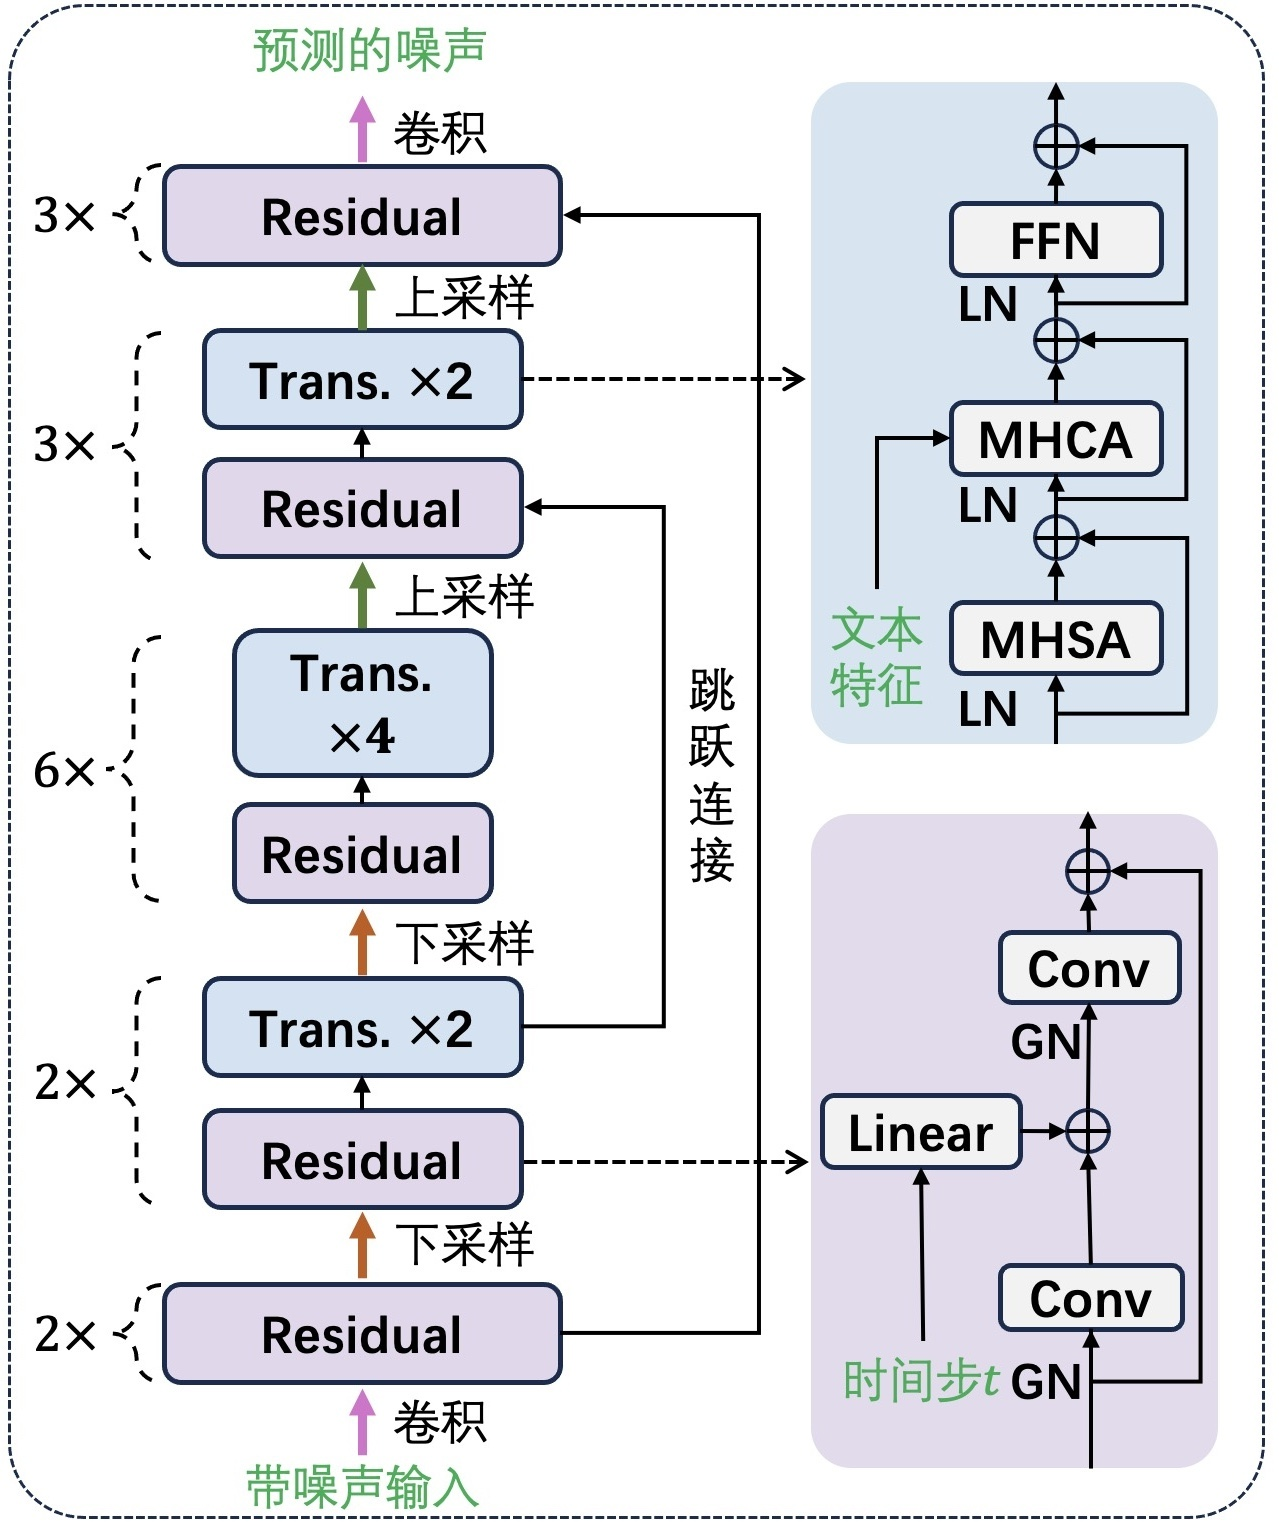
\includegraphics[width=\linewidth]{img/C-UNet.jpg}
        \caption{条件UNet}
        \label{fig:c-unet}
    \end{subfigure}
    \hfill
    \begin{subfigure}[b]{0.52\textwidth}
        \centering
        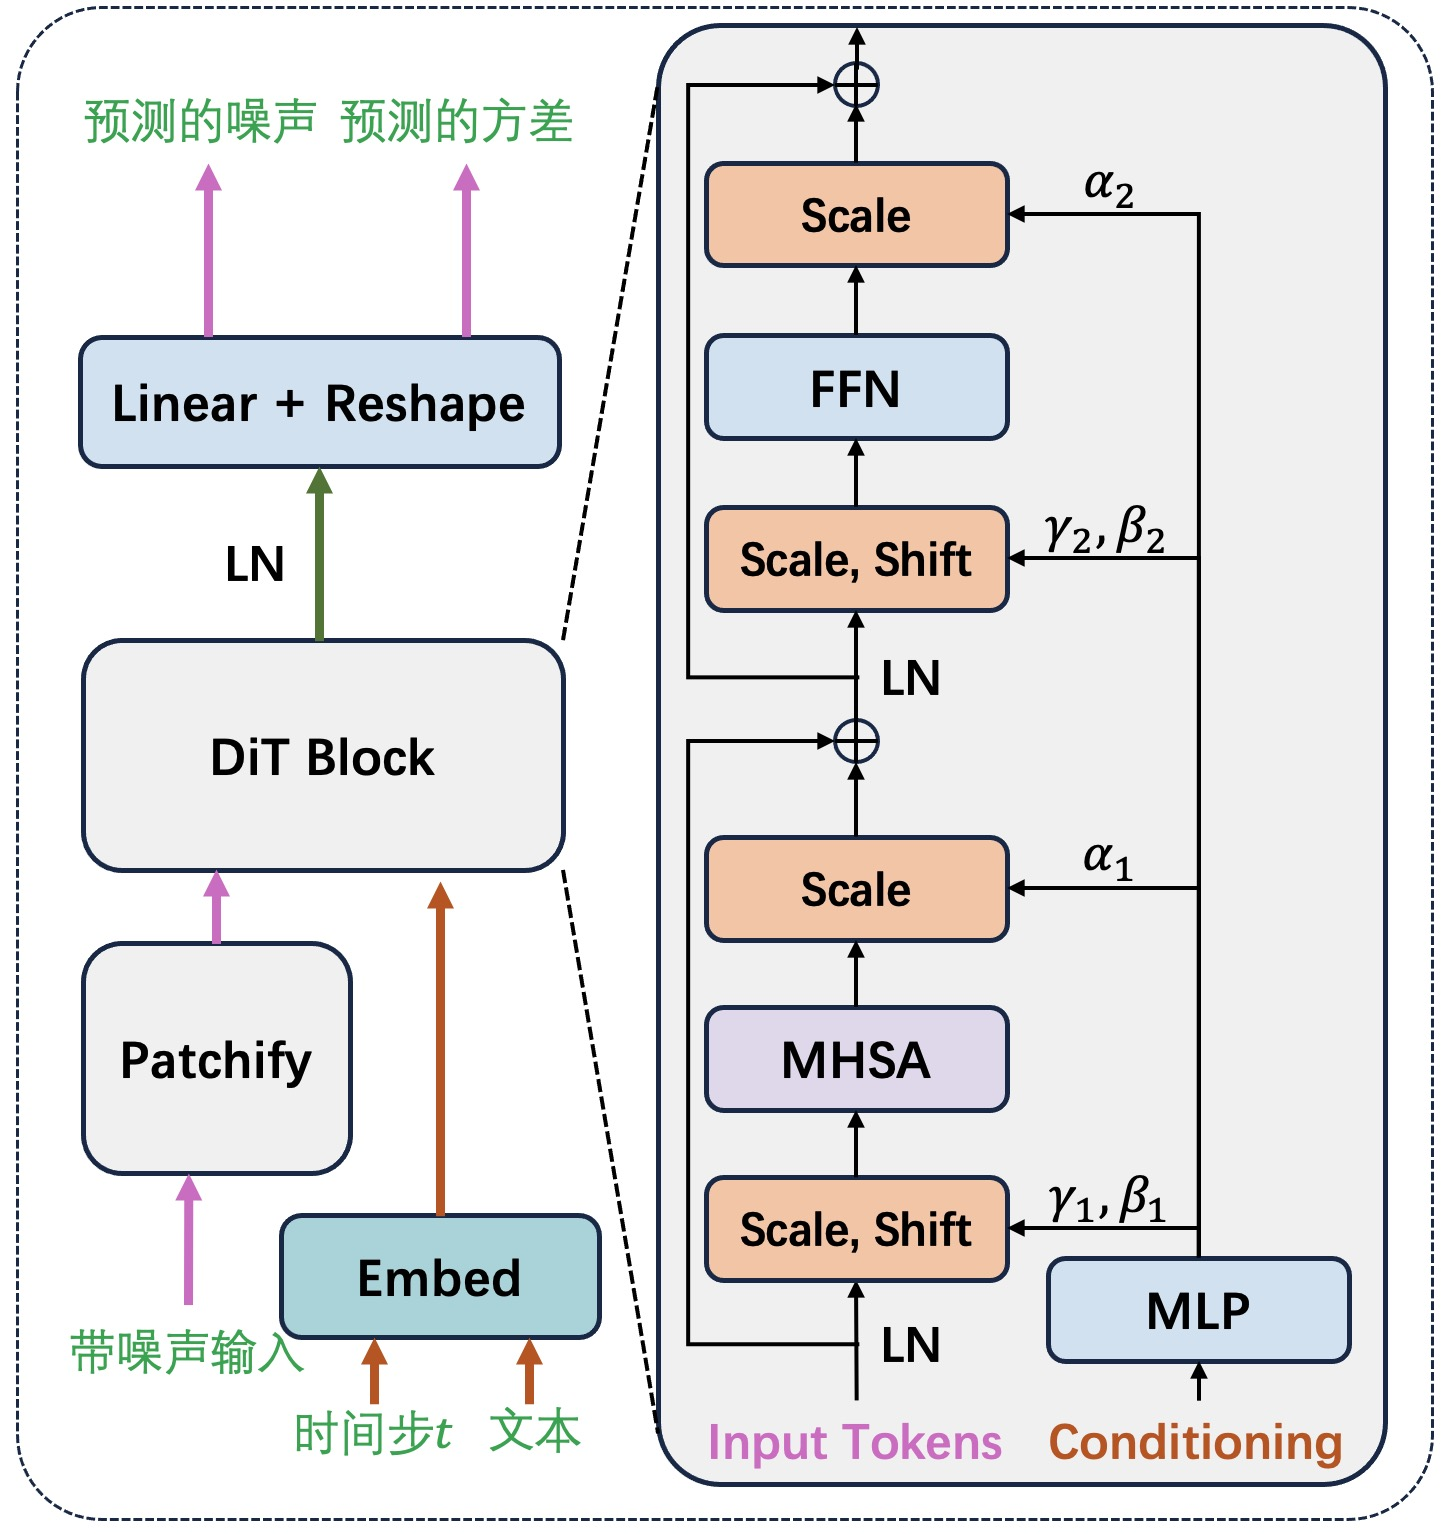
\includegraphics[width=\linewidth]{img/DiT.jpg}
        \caption{DiT}
        \label{fig:dit}
    \end{subfigure}
    \caption{条件UNet与DiT架构对比。关键模块说明——Residual:残差模块;Trans.:注意力模块;FFN/MLP/Linear:前馈网络(线性层);Conv:卷积层;LN:Layer Normalization;GN:Group Normalization;MHCA:多头交叉注意力层;MHSA:多头自注意力层;Patchify:分块编码;Embed:嵌入层}
    \label{fig:cunet-dit}
\end{figure}

在文本生成图像的扩散模型研究领域,架构设计的发展起到了至关重要的作用。早期的研究\cite{song2019generative,ho2020denoising}主要依赖于UNet架构\cite{ronneberger2015u}。UNet以卷积操作为核心,通过一系列下采样与上采样阶段,实现了从图像特征提取到重建的完整流程。具体而言,下采样阶段逐步降低图像空间分辨率,从而提取高层次语义信息;而上采样阶段则通过跳跃连接(skip connections)将低层次的空间细节与高层特征融合,有效恢复了图像的局部结构与纹理。中间阶段作为连接上下采样的桥梁,通常由多个处理单元构成,负责深层特征的转化与全局信息的整合。尽管UNet在多尺度去噪任务中表现出色,但其卷积操作受限于局部感受野,对长程依赖关系的建模能力有限。此外,UNet在外部条件信息(如文本提示)融合方面亦存在不足,从而一定程度上限制了其在文本到图像生成任务中的应用潜力。

为有效整合外部条件信息,研究者提出了多种创新方法。以GLIDE\cite{pmlr-v162-nichol22a}为例,该模型在UNet框架基础上通过双重机制引入文本信息:首先,利用Transformer对文本提示进行编码,将最终嵌入向量作为全局条件输入模型;其次,将文本token的中间层特征投影到UNet各注意力层,实现图像与文本特征在不同语义层次上的跨模态交互。Imagen\cite{saharia2022photorealistic}则采用预训练的文本编码器(如T5\cite{raffel2020exploring})生成语义嵌入,并在UNet结构中引入交叉注意力层,实现对文本与图像特征的动态对齐,同时将池化后的全局文本向量注入各级网络层,以保证语义一致性。在生成策略方面,GLIDE和Imagen均采用分层生成范式:先通过文本条件的扩散模型生成低分辨率图像,再借助超分辨率模块递进放大。DALL·E-2\cite{ramesh2022hierarchical}则创新性地结合CLIP文本编码器,先生成语义特征,再通过层级扩散模型合成高分辨率图像。尽管这些方法在文本与图像对齐方面取得了优异效果,但其级联式设计或对高分辨率图像的直接生成方式仍带来了较高计算成本的挑战。

针对上述问题,隐空间扩散模型(LDM)\cite{rombach2022high}为提升计算效率以及增强对长程依赖和外部条件信息的建模能力,提出了全新的解决方案。LDM在继承UNet多级上下采样结构与跳跃连接等核心设计的基础上,创新性地引入了自注意力和交叉注意力机制:前者用于捕捉图像内部全局依赖,后者实现对外部文本条件的高效控制。同时,LDM通过在残差块中融合时间步信息,进一步增强了对扩散过程动态的建模能力。这种为UNet注入条件信息的范式被后续大量工作采用,并成为Stable Diffusion系列模型的基础,在后文中,我们用\textbf{条件化UNet}(Conditional UNet)来指代此网络结构。随着模型参数规模的不断增大及训练策略的持续优化(如SDXL\cite{podell2023sdxl}),该架构的性能得到了极大提升,迅速成为学术界和工业界的主流选择之一。我们在图\ref{fig:c-unet}中展示了条件化UNet的结构。

近年来,随着视觉Transformer(ViT)\cite{dosovitskiy2020image} 的兴起,研究者们开始探索更为高效简洁的架构设计。例如,UViT\cite{uvit}将Transformer模块引入条件化UNet架构的中间阶段,取代传统卷积层,显著增强了模型的全局特征建模能力。尽管自注意力机制理论上计算复杂度较高,Transformer与MLP模块却能充分利用现代GPU/TPU的并行计算资源,使得实际应用中的效率依然可观。由于UViT的结构与条件化UNet高度相似,本文后续将其视为条件化UNet的一种变体,并将两者合并进行讨论。

Diffusion Transformer(DiT)\cite{peebles2022scalable} 则把扩散模型架构推向了新的方向。DiT完全摒弃了传统卷积结构,采用分块化输入处理方式——将图像切分为不重叠的patch序列,既保留了Transformer对序列数据的强大建模能力,又减轻了高分辨率输入带来的计算压力。其核心DiT Block以标准Transformer Block为基础(多头注意力加前馈网络),创新性地融入自适应层归一化(adaLN-Zero),通过将时间步与文本提示的特征作为条件输入,实现对扩散过程时序动态的精细调控。最终,解码器将处理后的token特征转回噪声和协方差预测,顺利完成生成流程。这些设计创新不仅大幅提升了图像生成质量和效率,也为扩散模型架构的未来发展开辟了新方向。我们在图\ref{fig:dit}中展示了DiT的结构。

稳定扩散模型(Stable Diffusion Models,SDMs)\cite{rombach2022high}是T2I合成领域最著名的开源模型之一,其卓越的生成能力已开始作为核心架构被应用于多项文本引导的视觉任务\cite{blattmann2023videoldm,brooks2023instructpix2pix,wang2023score,zhang2023adding}。SDMs本质上是专精于T2I的潜在扩散模型(LDMs)\cite{rombach2022high},通过在语义压缩空间执行扩散过程\cite{ho2022classifier,liu2021pseudo,song2020denoising}来提升计算效率。该模型可采用条件UNet或DiT架构对随机潜在编码进行迭代采样去噪,并配合文本编码器\cite{radford2021learning}与图像解码器\cite{esser2021taming,van2017neural}生成文本对齐的图像。我们在图\ref{fig:sdm}中展示了SDM的结构以及推理结构。

\begin{figure}[htbp]
\centering
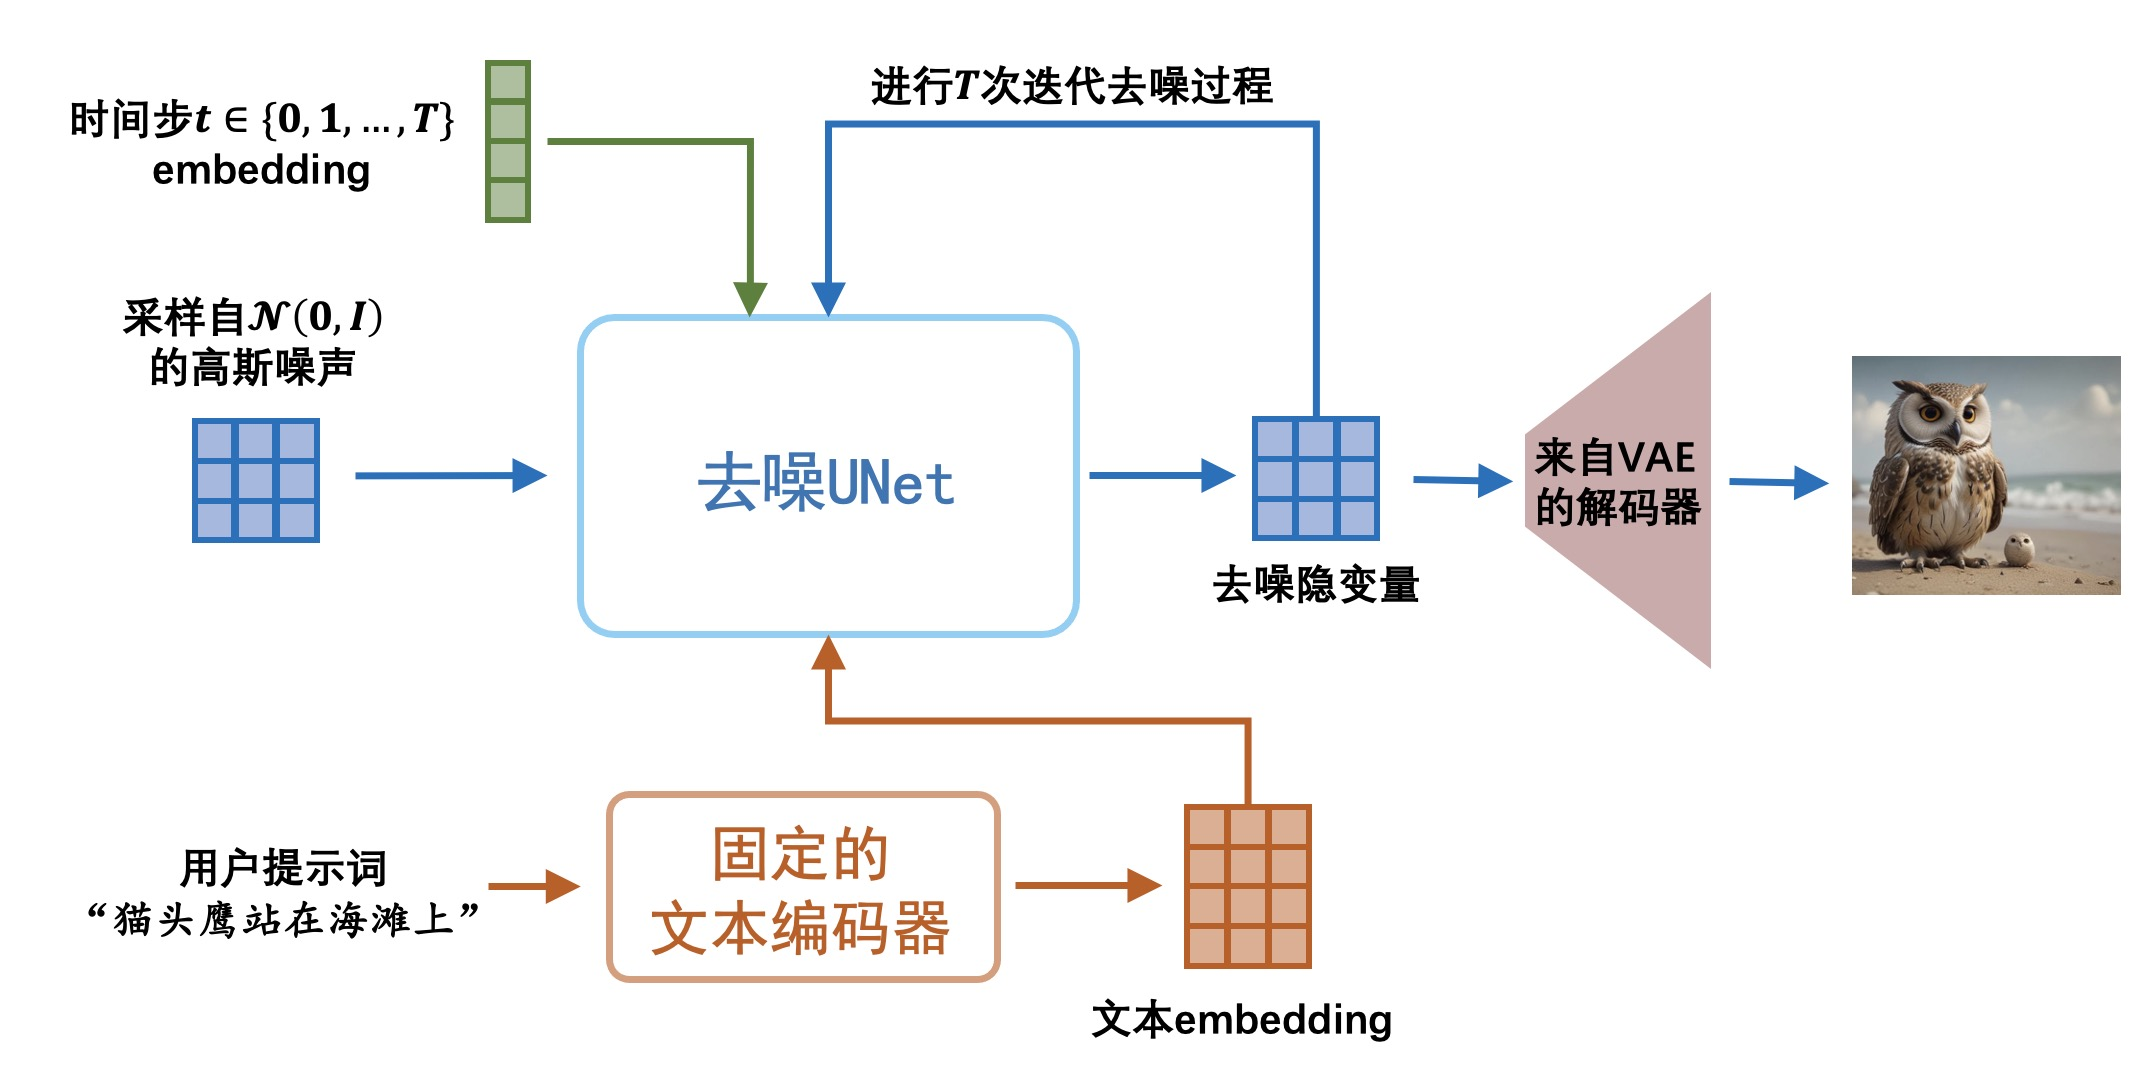
\includegraphics[width=0.8\textwidth]{img/SDM.jpg}
\caption{稳定扩散模型(SDM)的推理过程}
\label{fig:sdm}
\end{figure}

下面我们先阐述SDM的文生图的详细过程,随后介绍SDM中核心的去噪UNet网络的结构。SDM的文生图过程如图\ref{fig:sdm}所示,它是一个多阶段的生成流程:首先,用户输入的文本提示通过预训练且冻结的CLIP文本编码器转换为文本条件表征;与此同时,模型从标准高斯分布$\N(\mathbf{0},\mathbf{I})$采样初始噪声隐变量,并将离散时间步$t\in\{0,1,\cdots,T\}$编码为连续的时间步嵌入向量。这些信息(文本表征、噪声隐变量和时间步嵌入)共同输入到条件去噪UNet中,该网络通过$T$次迭代在文本条件的引导下逐步修正隐变量——每次迭代预测当前噪声并更新隐变量,使其逐渐逼近目标语义对应的隐空间分布。最终,优化后的隐变量通过VAE解码器映射到像素空间,生成符合用户需求的高分辨率图像。



\newpage

\iffalse
稳定扩散模型(Stable Diffusion Models,SDMs)\cite{rombach2022high}是T2I合成领域最著名的开源模型之一,其卓越的生成能力已开始作为核心架构被应用于多项文本引导的视觉任务\cite{blattmann2023videoldm,brooks2023instructpix2pix,wang2023score,zhang2023adding}。SDMs本质上是专精于T2I的潜在扩散模型(LDMs)\cite{rombach2022high},通过在语义压缩空间执行扩散过程\cite{ho2022classifier,liu2021pseudo,song2020denoising}来提升计算效率。该模型采用U-Net架构\cite{ronneberger2015u,dhariwal2021diffusion}对随机潜在编码进行迭代采样去噪,并配合文本编码器\cite{radford2021learning}与图像解码器\cite{esser2021taming,van2017neural}生成文本对齐的图像。

\begin{figure}[htbp]
    \centering
    \begin{subfigure}[b]{0.49\textwidth}
        \centering
        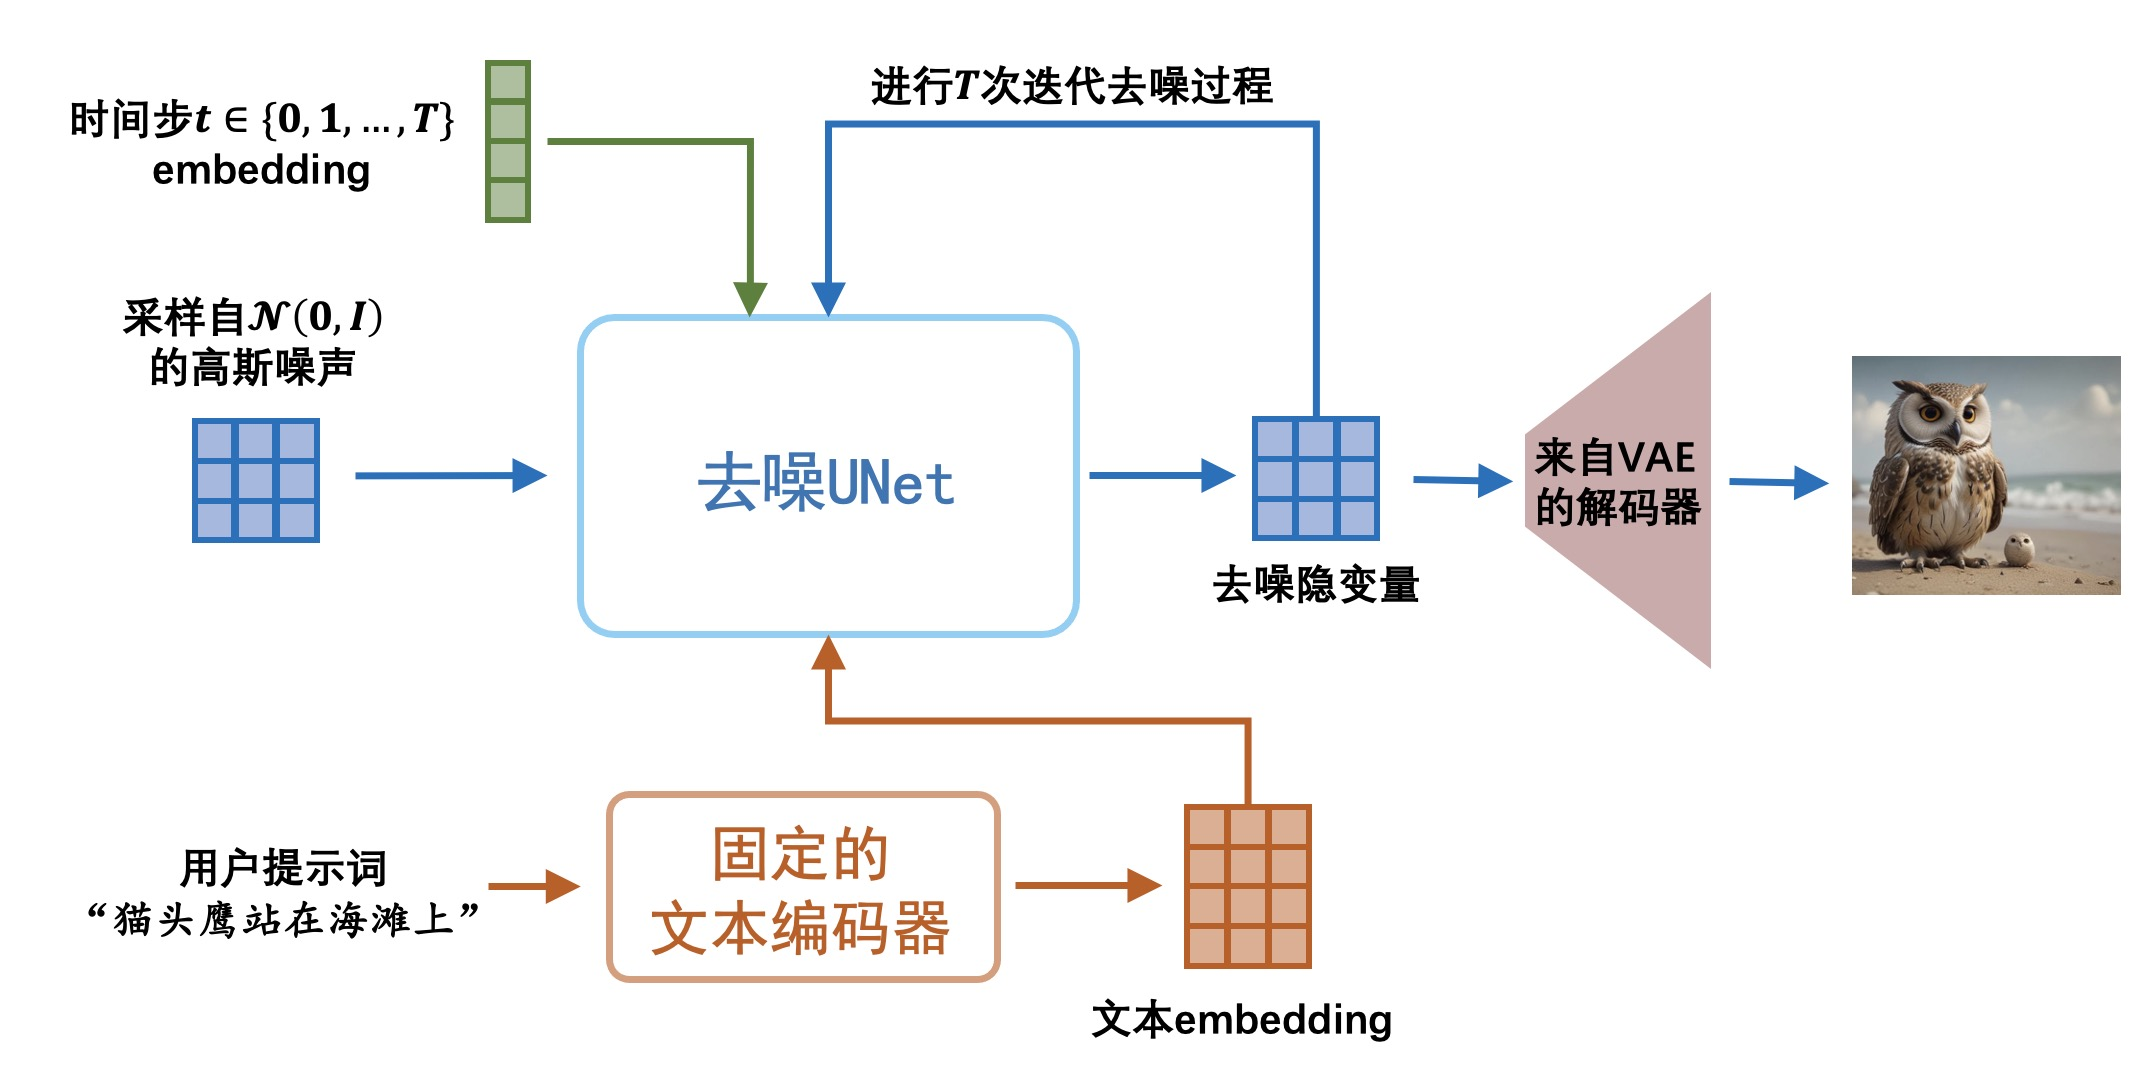
\includegraphics[width=\linewidth]{img/SDM.jpg}
        \caption{稳定扩散模型(SDM)的推理过程}
        \label{fig:sdm}
    \end{subfigure}
    \hfill
    \begin{subfigure}[b]{0.49\textwidth}
        \centering
        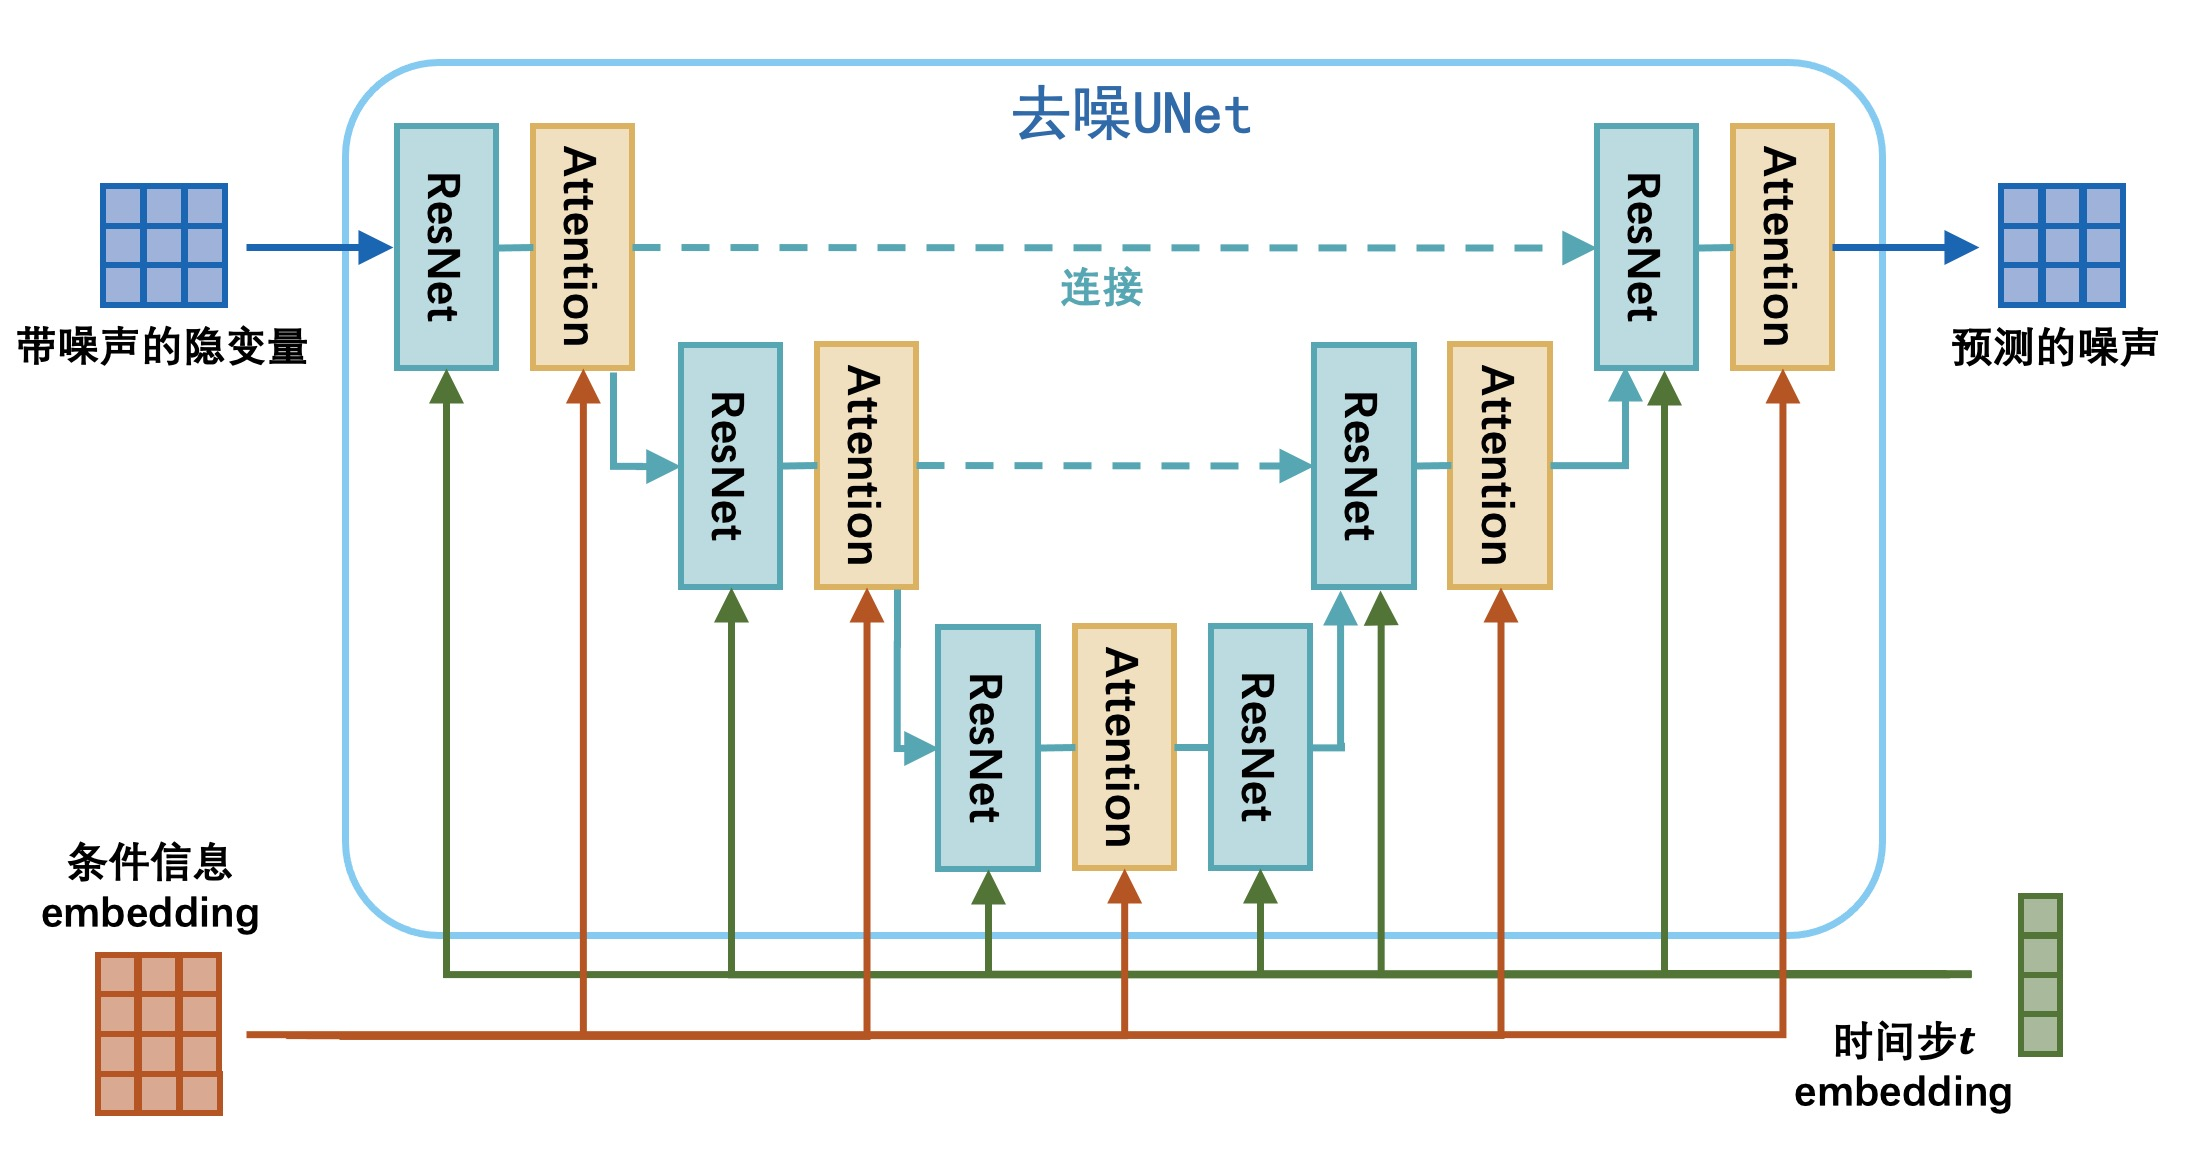
\includegraphics[width=\linewidth]{img/denoising-unet.jpg}
        \caption{去噪UNet的网络结构}
        \label{fig:unet}
    \end{subfigure}
    \caption{稳定扩散模型的推理与结构}
    \label{fig:sdm&unet}
\end{figure}

下面我们先阐述SDM的文生图的详细过程,随后介绍SDM中核心的去噪UNet网络的结构。SDM的文生图过程如图\ref{fig:sdm}所示,它是一个多阶段的生成流程:首先,用户输入的文本提示通过预训练且冻结的CLIP文本编码器转换为文本条件表征;与此同时,模型从标准高斯分布$\N(\mathbf{0},\mathbf{I})$采样初始噪声隐变量,并将离散时间步$t\in\{0,1,\cdots,T\}$编码为连续的时间步嵌入向量。这些信息(文本表征、噪声隐变量和时间步嵌入)共同输入到条件去噪UNet中,该网络通过$T$次迭代在文本条件的引导下逐步修正隐变量——每次迭代预测当前噪声并更新隐变量,使其逐渐逼近目标语义对应的隐空间分布。最终,优化后的隐变量通过VAE解码器映射到像素空间,生成符合用户需求的高分辨率图像。

去噪UNet结构如图\ref{fig:unet}所示,它采用了经典的编码器-解码器设计,形成对称的U形结构,其核心由多层ResNet模块和注意力机制组成。该网络接收带噪声的隐变量作为输入,通过左侧编码器部分的ResNet和Attention模块进行特征提取和降采样,同时文本表征和时间步嵌入被输入到各层模块中提供上下文信息;在U形结构底部达到最深特征表示后,右侧解码器部分通过ResNet和Attention模块进行特征重建和上采样,而图中虚线表示的连接机制将编码器对应层的特征直接传递到解码器对应层,有效保留细节信息。整个计算流程形成了一个端到端的噪声预测网络,最终输出预测的噪声,这种结合条件信息和时间步信息的架构设计使得去噪UNet能够有效学习噪声分布特征,在扩散模型等领域展现出优异性能。
\fi

\subsection{训练数据准备}


\subsection{模型测试基准}


\newpage



在下面介绍SDM的主流加速方法之前,我们先系统剖析SDM各个步骤的计算特征、参数分布及延时特性,为后续讨论奠定基础。这里我们主要使用来自Li等人在\cite{li2023snapfusion}中呈现的结果。他们对Stable Diffusion v1.5(SD-v1.5)\footnote{https://huggingface.co/stable-diffusion-v1-5/stable-diffusion-v1-5}模型各层的参数量与计算量展开全面研究。这项深度分析有助于从网络架构与算法范式的角度,理解文生图扩散模型在移动设备上部署的核心瓶颈。


\begin{figure}[htbp]
    \centering
    \begin{subfigure}[b]{0.49\textwidth}
        \centering
        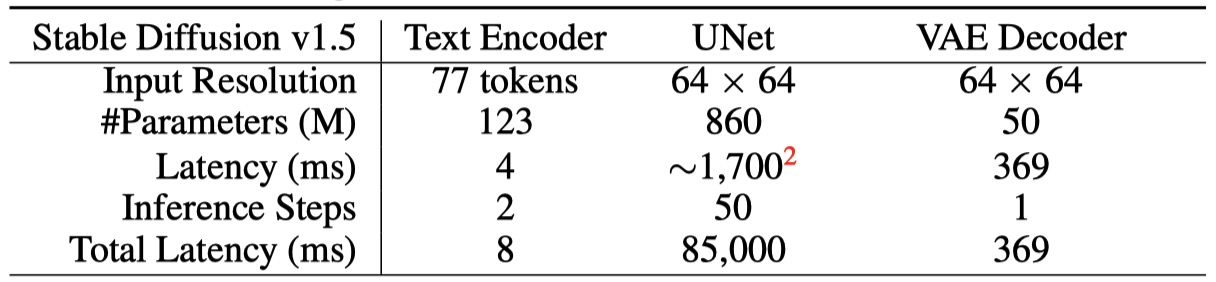
\includegraphics[width=\linewidth]{img/sdv15_latency.jpg}
        \caption{SD-v1.5模型中各模块在iPhone 14 Pro上的延时(ms)}
        \label{fig:latency_three}
    \end{subfigure}
    \hfill
    \begin{subfigure}[b]{0.49\textwidth}
        \centering
        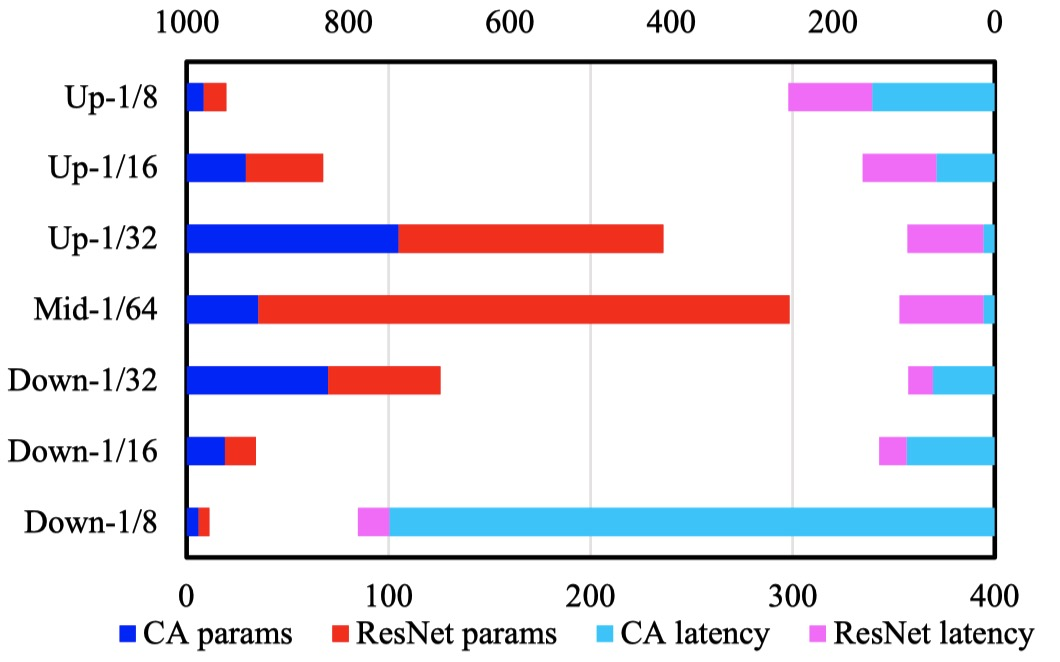
\includegraphics[width=\linewidth]{img/unet_latency_params.jpg}
        \caption{SD-v1.5中去噪UNet各层在iPhone 14 Pro上的延时(ms)和参数量(M)比较}
        \label{fig:latency_params_unet}
    \end{subfigure}
    \caption{SD-v1.5的延时与参数量分析}
    \label{fig:sd_v15}
\end{figure}

正如图\ref{fig:sdm}所展示的那样,SDM主要包含三个主要模块:文本编码器、去噪UNet和VAE解码器。图\ref{fig:latency_three}展示了这三个模块各自的参数量和延时。SD-v1.5中文本编码器是ViT-H模型\cite{radford2021learning}。由于该文生图模型采用无分类器引导,所以由(\ref{conditional_classifier_free_guided})可知,该文本编码器在生成每张图片时执行2次(一次输入为文本提示词输出条件表征,一次输入空串输出无条件表征),该部分仅占推理延迟的极小一部分(8毫秒)。VAE解码器负责将潜在特征生成图像,运行时延为369毫秒。与前两者不同的是,去噪UNet计算量极大(单步延迟为1.7秒),并且需要多次迭代前向传播以保证生成质量。

下面我们对去噪UNet的内部结构进行解析。该网络的内部结构如图\ref{fig:unet}所示,网络的核心是(交叉)注意力模块和ResNet模块。交叉注意力模块的作用是在每个阶段将文本信息融合到图像信息中,具体计算方式为:
\begin{equation*}
    \text{Cross-Attention}(Q_{\z_t},K_{\c},V_{\c})=\text{Softmax}\left(\frac{Q_{\z_t}\cdot K_{\c}^{\top}}{\sqrt{d}}\right)\cdot V_{\c},
\end{equation*}
其中$Q_{\z_t}$投影自噪声数据$\z_t$,$K_{\c}$和$V_{\c}$投影自文本信息$\c$,$d$是特征维度。ResNet模块在UNet中用于捕捉局部空间特征。ResNet与交叉注意力的结合,正是扩散模型兼顾全局语义与局部真实性的关键设计。图\ref{fig:latency_params_unet}对比了该网络各层的延时与参数量,可以看出参数主要集中在UNet中段,这是由于通道维度的扩展所致,其中ResNet块占据了绝大部分比例。相比之下,UNet中速度最慢的部分是输入和输出阶段,这些层级具有最大的特征分辨率,因为空间交叉注意力的计算复杂度与特征尺寸(在ViT中被量化为token数量)呈平方关系。

\newpage

\section{端侧部署的关键技术}

在本节中,我们将深入分析基于广泛应用的扩散模型(SDM)的主流加速方法。首先,我们将介绍\textbf{网络参数量化技术},这类方法在不显著修改网络架构的前提下,有效降低了计算内存和存储需求。随后,我们探讨多种\textbf{精简网络架构设计}的工作,它们通过不同策略简化网络结构以提高效率。由于修改网络架构后通常需要对模型进行微调,我们进而分析主流的\textbf{知识蒸馏与步数蒸馏}技术,其中知识蒸馏使小模型能够快速掌握大模型的能力,而步数蒸馏则大幅加速推理过程。最后,我们考察各种\textbf{底层计算优化方法},这些方法从硬件系统层面对扩散模型中的计算过程进行优化,进一步提升性能。

\subsection{网络参数量化技术}

在扩散模型加速领域,网络参数量化技术凭借其无需显著修改网络架构的特性,展现出独特优势。与高效架构设计和网络剪枝等方法相比,量化技术通过将浮点权重转换为低位固定点表示\cite{gholami2022survey,jin2022fnet},既保持了预训练模型的结构完整性,又有效降低了计算内存和存储需求。现有量化方法主要分为训练后量化(Post-Training Quantization,PTQ)和量化感知训练(Quantization-Aware Training,QAT)两大类。下面我们将分别介绍这两类方法的典型工作。

训练后量化(PTQ)技术因其部署便捷性受到研究者广泛关注。这类方法仅需少量校准数据即可完成量化参数调整,避免了耗时的完整重训练流程。然而,扩散模型特有的数据分布随时间变化特性对传统PTQ方法提出了挑战。为解决这一问题,研究者提出了多种创新解决方案:PTQ4DM\cite{shang2023post}提出基于偏态正态分布的时间步校准方法(NDTC),通过动态生成多时间步校准样本,实现了8位量化模型与全精度模型相当的性能;Q-Diffusion\cite{li2023q}设计了时间步感知校准和残差连接层分块量化策略,首次在4位量化条件下保持了扩散模型的稳定性能;PTQD\cite{he2023ptqd}通过量化噪声解耦,分别采用相关系数校正和方差调度校准技术进行补偿,同时引入基于步骤感知的混合精度策略,在保持生成质量的同时显著减少了计算需求;TDQ\cite{so2023temporal}提出了基于时间步信息的动态量化方法,通过可学习的时序感知模块自适应生成最优量化配置;TFMQ\cite{Huang_2024_CVPR}则针对时序特征失真问题,提出了独立于输入数据的时序信息块,结合时序感知重建和有限集校准技术,在4比特量化下实现了接近全精度模型的生成质量。

尽管PTQ方法操作高效,但在极低位宽(如4位及以下)量化时往往引入显著误差,甚至导致模型完全丧失去噪能力\cite{he2023ptqd}。量化感知训练(QAT)\cite{krishnamoorthi2018quantizing,esser2019learned}虽然可通过全模型微调恢复低位性能,但其计算开销通常远超PTQ方法。为平衡效率与性能,研究者提出了一系列折中方案:EfficientDM\cite{he2024efficientdm}结合LoRA框架\cite{hu2022lora}提出量化感知低秩适配器(QALoRA),实现了权重与激活的联合低比特量化,在保持PTQ级效率的同时达到QAT级的生成质量;Q-DM\cite{li2023qdm}针对激活分布振荡和量化误差累积问题,提出了时间步感知量化(TaQ)和噪声估计模仿(NeM)技术;BitsFusion\cite{sui2024bitsfusion}通过分析各层量化敏感性并设计分层位宽分配策略,结合时间嵌入预计算缓存、平衡整数初始化及交替优化缩放因子等技术,将Stable Diffusion v1.5的UNet有效压缩到平均1.99比特。

这些进展表明,扩散模型量化技术正朝着更低位宽、更高效率、更小精度损失的方向快速发展,为端侧部署提供了重要技术支持。我们在图x中详细展示了这些方法的技术细节。

【这里可以加一张表,每行表示一种方法,可以分PTQ和QAT两大类;每列表示该方法的一种属性,比如方法被提出的时间、量化比特宽度(随不同方法下降所能保持的模型质量,如4/8bit等)、推理效率、生成质量、部署便利、关键技术等】

\subsection{精简网络架构设计}

\iffalse
在文本生成图像的扩散模型研究领域中,架构设计的发展起到了至关重要的作用。早期的研究工作\cite{song2019generative, ho2020denoising},主要依赖于UNet架构\cite{ronneberger2015u}。该架构以卷积操作为核心,通过一系列下采样和上采样阶段实现了从图像特征提取到图像重建的过程。具体而言,下采样阶段逐步降低了图像的空间分辨率,同时提取了高层次的语义信息;相反地,在上采样阶段,通过跳跃连接(skip connections)将低层次的空间细节与高层特征相结合,有效地恢复了图像的局部结构与纹理。中间阶段作为上下采样过程中的桥梁,通常由多个处理单元组成,负责深层次的特征转换与全局信息整合。尽管UNet在多尺度去噪任务中表现出色,但其基于局部感受野的卷积操作限制了对长程依赖关系的建模能力,并且未能有效结合外部条件信息,如文本提示,这在一定程度上限制了其在文本到图像生成任务中的应用。

为解决上述问题,隐空间扩散模型(LDM)\cite{rombach2022high}提出了一种新的解决方案,旨在提升计算效率的同时增强对长程依赖关系以及外部条件信息的建模能力。LDM在继承UNet的多级上下采样结构和跳跃连接等核心设计的同时,创新地引入了注意力机制,特别是自注意力层和交叉注意力层的设计,前者用于捕捉图像内部的全局依赖关系,后者则实现了对外部文本条件的有效控制。此外,通过在残差块中融合时间步信息,LDM进一步增强了模型的时间动态建模能力。这种“条件化UNet”的范式被后续的工作广泛采用,并成为Stable Diffusion系列模型的基础。随着参数量的增加和训练策略的改进,例如SDXL\cite{podell2023sdxl},该架构的性能得到了显著提升,逐渐成为了学术界和工业界的主流选择之一。

近年来,随着视觉Transformer(ViT)\cite{dosovitskiy2020image} 的兴起,研究者们开始探索更加高效简洁的架构设计。UViT\cite{uvit} 便是这一趋势下的产物,它将Transformer模块应用于条件化UNet架构的中间阶段,取代了原有的卷积层,从而增强了模型的全局特征表示能力。尽管自注意力机制理论上具有较高的计算复杂度,但由于Transformer和MLP模块能够充分利用现代GPU/TPU的并行计算能力,因此在实际应用中仍能保持较高的计算效率。

Diffusion Transformer(DiT)\cite{peebles2022scalable} 则代表了扩散模型架构设计的新方向,它完全放弃了传统的卷积结构。DiT采用了分块化的输入处理方法,将图像转换为非重叠的patch序列,这样既保留了Transformer处理序列数据的优势,又解决了高分辨率图像带来的计算挑战。核心模块DiT Block在保留标准Transformer Block(多头注意力机制+前馈网络)基本架构的同时,创新性地引入了自适应层归一化层(adaLN-Zero),该模块通过将时间步和文本提示词的特征向量作为条件输入,实现了对扩散过程时序动态的精确建模。最终,通过一个轻量级解码器将处理后的token特征转换回预测的噪声与协方差,完成了整个生成流程。这些创新使得DiT在提高图像生成质量和效率方面取得了显著进展,展示了扩散模型架构发展的新前景。
\fi


【针对UNet(LDM)的改进】

针对上述问题,BK-SDM\cite{kim2023bk}提出了一种基于敏感度分析的分阶段剪枝策略。该方法首先在下采样阶段采用选择性剪枝策略,系统性地移除冗余的残差-注意力模块对,仅保留每个分辨率阶段的首组模块以处理关键的空间信息变换;同时在上采样阶段保留每个分辨率阶段的末组模块,确保跳跃连接的有效性。其次,通过实验验证发现中间阶段具有较高的冗余度,完全移除后对生成质量影响甚微。为验证剪枝策略的合理性,研究采用模块重要性评估方法,通过量化移除单个模块后生成性能的下降幅度来判定其重要性。实验结果表明,该策略在保持生成质量的同时,显著减少了30\%-50\%的参数量,有效实现了计算效率与模型性能的优化平衡。

BK-SDM\cite{kim2023bk}在训练剪枝模型时采用了创新的多目标联合训练框架:首先通过标准去噪损失函数维持模型的基础图像生成能力;其次引入输出级知识蒸馏损失,确保学生模型与教师模型的预测结果保持一致;同时设计了特征级知识蒸馏,通过在对应UNet阶段末端直接进行特征对齐。这种多层级蒸馏机制有效实现了轻量化学生模型对原始教师模型行为的精确模仿。

EdgeFusion\cite{castells2024edgefusion}在BK-SDM轻量化架构的基础上,通过引入合成的高质量图文对齐数据集显著提升了模型的生成性能。该方法进一步结合潜在一致性模型(LCM)的步骤蒸馏技术,实现了仅需少量推理步骤即可生成高质量图像的效果。

为了在保持预训练UNet模型性能的同时提升其效率,同时避免因架构变动导致的性能退化问题,SnapFusion\cite{li2023snapfusion}提出了一种创新的架构演化方法。该方法首先采用鲁棒训练框架,通过在训练过程中随机跳过特定模块(如交叉注意力或ResNet块),使网络能够适应不同的模块组合,从而增强其对架构变动的鲁棒性。基于这一训练框架,该方法进一步设计了系统的架构优化策略:通过构建包含添加/删除模块操作的演化动作集,并引入量化评估指标($\frac{\Delta\text{CLIP}}{\Delta\text{Latency}}$)来精确衡量每个模块对模型性能和效率的贡献度。其中,具有较高$\frac{\Delta\text{CLIP}}{\Delta\text{Latency}}$比值的模块将被优先保留,而贡献度较低的冗余模块则会被动态移除,最终在无需额外微调的情况下实现模型效率的显著提升。在图像解码器优化方面,该方法首先对原始网络通道进行结构化裁剪,获得轻量化模型架构;随后以SD-v1.5作为教师模型,通过知识蒸馏技术将大模型的生成能力迁移至该小模型。

SnapFusion\cite{li2023snapfusion}提出了一种高效的扩散模型优化框架,其核心包含两个关键创新:首先,该方法采用$\v$预测($\v$-prediction)模式对UNet进行微调,通过建模噪声$\epsilon$与无噪声隐变量$\x$的线性组合$\v=\alpha_t\epsilon-\sigma_t\x$,显著提升了梯度传播的平滑性和多步去噪过程的稳定性;其次,创新性地提出了CFG(classifier-free guidance)感知的步数蒸馏策略,该策略通过动态调节分类器引导系数,在保持生成质量的同时实现生成多样性的灵活控制。基于渐进式蒸馏的思想,该方法最终将50步的原始模型高效压缩为仅需8步推理的轻量UNet模型,在保证生成质量的前提下实现了显著的加速效果。

【针对U-ViT的改进】

Hu等人\cite{hu2024snapgen}提出轻量化扩散模型SnapGen,通过多项架构创新实现移动端高效文本生成图像。主要技术包括:(1)精简注意力机制,仅保留最低分辨率层的自注意力;(2)采用扩展可分离卷积\cite{howard2017mobilenets}模块,平衡计算效率与模型性能;(3)使用多查询注意力(MQA)\cite{shazeer2019fast}替代传统多头自注意力(MHSA),显著减少参数;(4)优化条件注入方式,在UNet首阶段引入交叉注意力;(5)精简FFN结构降低计算开销;(6)采用QK RMSNorm\cite{henry2020query,zhang2019root}防止softmax饱和并加速收敛,结合二维RoPE编码\cite{su2024roformer}消除高分辨率生成中的物体重复问题,两者计算开销几乎可忽略。这些技术使得该模型仅需0.38B参数即可在移动端实现1024×1024分辨率图像的快速生成。针对高分辨率图像生成中的解码器效率瓶颈,该研究通过移除注意力层、精简归一化层、采用深度可分离卷积等轻量化设计,显著降低了移动端部署时的内存占用。

SnapGen\cite{hu2024snapgen}通过三阶段训练策略显著提升了轻量化扩散模型的生成质量:首先采用修正流(RF)\cite{liu2022flow}构建线性传输路径,结合logit-normal时间步采样和Flow-Euler推理算法,优化了高分辨率图像的生成效果;其次提出多层级知识蒸馏框架,通过输出级速度场对齐、跨架构特征匹配和时间步感知动态加权,实现了教师模型(SD3.5-Large)到学生模型的高效知识迁移;最后引入基于LADD框架\cite{sauer2024fast}的步数蒸馏技术,将扩散模型与GAN的对抗训练相结合,使轻量化模型仅需少量去噪步即可达到Turbo级模型的生成质量。

MobileDiffusion\cite{zhao2024mobilediffusion}方法采用UViT网络,并对Transformer和卷积这两个基础模块进行系统研究以加速计算。针对Transformer模块的优化主要包括:(1)在UViT主干网络中增加transformer层数并降低通道维度,保持参数量不变的同时提升计算效率;(2)高分辨率层移除自注意力但保留交叉注意力,兼顾效率与性能;(3)自注意力层的key和value共享投影矩阵以减少参数;(4)用Swish替换GELU,提升计算稳定性;(5)将softmax注意力替换为ReLU,仅需少量微调即可适配;(6)精简前馈层结构,在减少参数量的同时保持模型性能。针对卷积模块,该方法通过将除最外层外的所有卷积层替换为可分离卷积\cite{howard2017mobilenets}、并剪枝冗余的残差块进行优化。此外,针对图像解码器模块,该方法首先通过结构剪枝(调整网络宽度和深度)构建轻量化架构,随后在微调阶段移除KL正则化项并降低对抗损失权重,最终实现解码速度实现3倍的提升。

在模型微调方面,MobileDiffusion\cite{zhao2024mobilediffusion}采用对抗微调与参数高效适配相结合的技术路线:一方面继承UFOGen\cite{xu2024ufogen}的生成器-判别器联合训练框架,通过对抗损失提升单步生成质量,同时保留扩散损失以维持特征空间稳定性;另一方面引入LoRA\cite{hu2022lora}微调机制,仅对生成器进行低秩矩阵更新,在保留预训练模型核心参数的同时实现高效适配。

Liu等人\cite{liu2024linfusion}针对扩散模型中自注意力层的二次计算复杂度问题,创新性地提出了LinFusion模块。该模块采用非因果归一化线性注意力机制,通过三个关键设计实现突破:首先,摒弃了传统序列建模中“当前状态只能依赖过去信息”的时序约束,建立任意位置间的直接交互机制,实现全局上下文的并行处理;其次,引入状态空间模型的隐式低秩投影技术,有效降低计算复杂度;最后,结合动态对角归一化(模拟softmax的概率分布特性),在保持注意力表达能力的同时将计算复杂度降至线性。在模型微调阶段,该方法仅需训练LinFusion模块参数,并创新性地结合噪声预测损失与双重知识蒸馏损失(分别对齐模型最终输出和层级特征)。这一工作实现了扩散模型中自注意力层的线性复杂度替代,为高清图像生成提供了新思路。【该模块可用于UNet或U-ViT】

【针对DiT的改进】

SANA\cite{xie2024sana}在DiT架构和LDM训练范式基础上进行了系统性创新:首先设计了更高压缩率的自编码器,显著提升了训练效率并支持超清图像生成;其次提出线性DiT架构,通过线性注意力替代原始自注意力提升计算效率,同时引入含3×3深度可分离卷积的Mix-FFN模块增强局部特征建模,实现了无位置编码(NoPE)设计;在文本理解方面,采用Gemma大语言模型\cite{team2024gemma}作为编码器,并基于其上下文学习能力设计了复杂人类指令(CHI)机制,大幅提升了提示词理解能力;最后通过多视觉语言模型协同标注优化训练数据,结合基于流的训练方法\cite{liu2022flow,karras2022elucidating}和Flow-DPM-Solver,在仅需14-20步推理采样的情况下仍保持优异生成质量。这些改进使模型在训练效率、推理速度和生成质量等方面均取得显著提升。

SANA\cite{xie2024sana}的边缘部署方案通过以下技术实现高效推理:首先采用混合精度量化策略,对网络激活值实施逐令牌对称INT8量化,权重采用逐通道对称INT8量化,同时保留交叉注意力块中的归一化层、线性注意力及KV投影层的FP16精度以确保语义保真度;其次通过核函数融合技术,将线性注意力的ReLU(K)TV运算与QKV投影层集成,并融合Mix-FFN中的GLU与量化核,同时合并其他逐元素操作,配合GEMM/Conv核的激活值布局优化和转置开销消除,显著提升了计算效率。这些优化在保证模型精度的同时大幅降低了计算和内存开销。


\subsection{知识蒸馏与步数蒸馏}

\textbf{渐进式蒸馏}: Salimans等人\cite{salimans2021progressive}提出的渐进式蒸馏(Progressive Distillation)框架通过迭代式知识迁移实现扩散模型的高效采样。该方法采用多阶段蒸馏策略:首先训练一个$N$步采样的基准模型作为教师模型,然后构建$N/2$步学生模型,通过最小化学生单步预测与教师两步预测的误差实现知识迁移。在迭代过程中,前轮学生模型作为新教师继续蒸馏更精简的模型,整个过程采用确定性DDIM\cite{song2020denoising}采样和特殊参数化方法确保稳定性,最终仅需4-8步即可达到原始模型数千步的采样质量。Meng等人\cite{meng2022distillation}针对无分类器引导(classifier-free guided)扩散模型,提出了一种两阶段蒸馏方法:第一阶段让学生模型学习教师模型的有条件与无条件加权输出,将教师模型多步计算压缩为单步的高效计算,并通过随机引导强度训练实现单一模型对多种引导强度的灵活适配。第二阶段采用渐进式蒸馏\cite{salimans2021progressive}将模型进一步压缩至1-4步采样,在保持生成质量的同时实现10-256倍加速。

\textbf{约束扩散轨迹的步数蒸馏}:在\ref{sec:rf_cm_lcm}小节中,我们系统性地介绍了三种基于轨迹优化的新型扩散模型范式:修正流(Rectified Flow, RF)\cite{liu2022flow}、一致性模型(Consistency Model, CM)\cite{pmlr-v202-song23a}和隐空间一致性模型(Latent Consistency Model, LCM)\cite{luo2023latent}。这些方法的共同特征是通过对扩散轨迹的几何性质进行约束或修正,显著简化了从噪声空间到数据空间的映射路径,从而实现了少步甚至单步的高效生成。值得注意的是,这些方法不仅可以独立构建生成模型,还能够作为有效的蒸馏框架,用于让预训练扩散模型具备的高效推理能力。

具体而言,修正流(RF)采用线性路径连接数据分布与噪声分布,通过速度场直接建模噪声到数据的确定性位移关系。该方法通过Flow-Euler采样器实现10-20步的高效生成,其核心优势在于摆脱了传统扩散模型对分数函数的依赖。一致性模型(CM)则提出了更具突破性的解决方案,其通过构建一致性函数将概率流ODE轨迹上的任意点直接映射至轨迹起点,并利用自一致性约束保证相邻时间步输出的稳定性,从而实现了单步生成的突破性进展。进一步地,隐空间一致性模型(LCM)通过将CM的一致性约束迁移到预训练扩散模型的隐空间,不仅保留了CM的高效生成特性,还显著降低了计算成本,为实际应用提供了更可行的解决方案。


\textbf{结合对抗学习的步数蒸馏}:

Sauer等人\cite{sauer2024adversarial}针对扩散模型因迭代采样导致推理速度慢的问题,提出了一种结合对抗训练与蒸馏的新方法——对抗扩散蒸馏(Adversarial Diffusion Distillation, ADD),该方法利用对抗损失确保单步生成的高保真度,同时通过蒸馏预训练扩散模型保留对复杂数据分布的建模能力。实验结果表明,该方法仅需1-4步采样即可达到与SDXL\cite{podell2023sdxl}等先进扩散模型相媲美的生成质量。

隐空间对抗扩散蒸馏(Latent Adversarial Diffusion Distillation,LADD)\cite{sauer2024fast}在对抗扩散蒸馏(ADD)基础上进行了重要改进。它将教师和学生模型操作转移到隐空间,降低计算成本的同时提升了对高分辨率和多尺度图像的支持能力,并兼容大规模模型架构。LADD还创新性地使用教师模型提取的隐空间多尺度特征计算对抗损失,有效避免像素级对齐的过拟合风险,同时增强了跨模态应用的灵活性。

UFOGen\cite{xu2024ufogen}通过新颖的扩散-GAN联合优化目标,实现了单步推理生成高质量文本条件图像的突破。该框架中的对抗损失专注于提升单步生成图像的视觉质量,使模型能够有效处理高噪声水平并产生更为锐利的细节;同时,扩散损失一方面稳定了对抗训练过程,为生成器提供明确的学习方向,另一方面有效保持了预训练扩散模型的特征完整性,从而确保生成内容的语义一致性和多样性。

\textbf{基于分布匹配的步数蒸馏}:

分布匹配蒸馏(Distribution Matching Distillation,DMD)\cite{yin2024one}的核心目标是将多步扩散模型蒸馏成一个单步生成器,在保持高质量图像生成能力的同时大幅提升推理速度。该方法的核心是结合分布匹配和回归正则化:首先利用真实/伪数据扩散模型计算能使生成图像靠近真实数据分布而远离伪数据分布的梯度方向,引导生成器输出更逼真的图像;同时通过预计算扩散模型的多步采样结果,采用LPIPS损失\cite{zhang2018unreasonable}强制单步生成器对齐教师模型的输出分布。这种双重优化机制实现了高效的单步高质量图像生成。

现有DMD方法虽通过分布匹配实现扩散模型蒸馏,但仍依赖回归损失保证训练稳定性,导致计算成本高昂且生成质量受限于教师模型。为此,DMD2\cite{yin2024improved}提出了一系列创新性改进:首先,通过引入判别器构建对抗训练框架,并采用两时间尺度更新规则(TTUR)优先优化判别器,使其快速收敛至最优状态,从而仅依靠判别器提供的可靠梯度信号即可确保训练稳定性,彻底摆脱了对回归损失的依赖;其次,在损失函数中引入对抗损失项,直接利用真实数据分布进行监督,显著提升了生成样本的质量;最后,创新性地设计了反向模拟训练策略,通过在训练过程中模拟多步推理的输入分布,有效解决了训练与推理阶段的分布不匹配问题。


\subsection{底层计算优化方法}

底层计算优化方法是指通过改进算法实现层面的计算效率、内存访问模式和硬件资源调度,从而在不改变模型数学架构的前提下提升性能的技术手段。这类方法通常涉及算子融合、内存布局优化、并行计算策略调整等细粒度操作,其核心在于充分利用硬件特性(如GPU的SIMT架构、缓存层次结构)来减少冗余计算和通信开销。在深度学习领域,此类优化常体现为定制化内核设计(如CUDA/OpenCL)、计算图重写(如TVM\cite{TVM}、TensorRT)以及编译器级优化(如MLIR\cite{mlir}),尤其对计算密集型任务(如扩散模型推理)具有关键作用。

Chen等人\cite{chen2023speed}针对移动端部署大型扩散模型的挑战,提出了一套GPU感知的底层优化方案。其核心技术包括:(1)通过为GroupNorm和GELU设计融合的GPU算子,减少内存搬运降低延迟;(2)结合部分Softmax融合与选择性FlashAttention\cite{dao2022flashattention}应用,更好地平衡了注意力机制的计算精度与效率;(3)通过Winograd卷积加速常规卷积操作。该方法为边缘设备高效运行十亿参数级扩散模型提供了可复用的底层优化范式。

EdgeFusion提出的模型级分块(Model-Level Tiling,MLT)方法通过将U-Net模型划分为更小的计算片段,以适配边缘NPU的内存限制。该方法动态优化分块策略,重点解决U-Net中残差块和注意力层的大规模特征图带来的DRAM访问瓶颈,同时最大化SRAM利用率。其创新性在于结合NPU硬件特性(如张量/向量引擎),通过计算SRAM需求自动配置分块参数,显著提升U-Net在边缘设备上的推理效率。

SANA提出通过Triton(Tillet et al., 2019)融合线性注意力前向/反向传播的核函数,将激活函数、精度转换等操作整合至矩阵乘法,减少数据传输开销。


\iffalse
\newpage

\subsection{优化模型结构与计算}

\subsubsection{简化模型计算}

BK-SDM(Block-removed Knowledge-distilled Stable Diffusion Model)是一种通过结构化剪枝与蒸馏训练协同优化的轻量化文本生成图像模型。其核心创新在于:1)基于敏感度分析定向剪除U-Net中冗余的残差-注意力模块对,在保持空间维度的前提下实现参数量减少30\%;2)采用多层级蒸馏损失函数(输出层+特征层对齐),使精简后的学生模型完美复现原始模型的去噪行为。该方法在三星NPU上实现了512×512图像的亚秒级生成,同时维持与完整模型相当的视觉质量。

SnapGen\cite{hu2024snapgen}通过精简Transformer块和通道维度,并移除高分辨率阶段的自注意力,显著了降低计算量且提升了性能。同时,该方法采用扩展可分离卷积(Separable Convolution)\cite{howard2017mobilenets}和多查询注意力(Multi-Query Attention)\cite{shazeer2019fast}分别替代普通卷积和多头自注意力,进一步提升了模型效率。

削减冗余参数:SnapFusion\cite{li2023snapfusion},BitsFusion\cite{sui2024bitsfusion}

SANA\cite{xie2024sana}和LinFusion\cite{liu2024linfusion}使用线性注意力\cite{cai2023efficientvit,dao2024transformers,katharopoulos2020transformers}

EdgeFusion\cite{castells2024edgefusion}提出了一种面向移动端的高效文本到图像生成框架,其创新性主要体现在三个关键技术维度。首先,该研究设计了一种两阶段知识蒸馏范式:第一阶段通过高质量教师模型优化轻量级学生模型,第二阶段结合潜在一致性模型(LCM)\cite{luo2023latent}进行微调,实现了仅需2-4步推理即可生成高质量图像的突破,在保持生成质量的同时显著提升了推理效率。其次,针对训练数据质量这一核心问题,研究团队创新性地采用GPT-4生成的文本描述与SDXL合成的图像构建高质量训练数据集,这一策略不仅提升了文本-图像语义对齐的准确性,还显著降低了传统LAION数据集存在的噪声干扰。最后,在硬件适配方面,研究提出了一套针对NPU的优化方案,包括创新的模型分块技术以优化内存访问效率、混合精度量化策略以平衡计算精度与效率,以及算子融合等加速技术。这些技术的协同创新使EdgeFusion成为首个能在移动设备上实现实时高质量图像生成的端到端解决方案。

MobileDiffusion\cite{zhao2024mobilediffusion}在网络架构设计上实现了显著的轻量化改进,其核心创新体现在层次化的结构优化策略。该模型在低分辨率特征层采用 Transformer模块以增强全局表征能力,同时在高分辨率层部署深度可分离卷积来降低计算复杂度。通过引入共享键值投影机制和解耦的自注意力/交叉注意力结构,有效减少了注意力模块的参数规模和计算延迟。进一步的优化包括采用Swish激活函数替代传统GELU,以及通过残差块剪枝实现模型压缩,最终在将参数量控制在0.4B以内的同时,仍保持了与Stable Diffusion v1.5相当的图像生成质量。

\subsubsection{通过知识蒸馏获得小模型}

将相同架构的大教室模型蒸馏为更紧凑、高效的学生模型\cite{kim2023bk,liu2024linfusion},这些方法通过移除注意力机制\cite{vaswani2017attention}或残差块\cite{he2016deep}等组件来降低模型复杂度,同时保持架构结构不变。

通过蒸馏训练使学生模型在更少步数内匹配教师模型样本质量:\cite{luo2023lcm},\cite{meng2023distillation},\cite{salimans2022progressive},\cite{song2023consistency}

通过蒸馏将模型评估次数缩减至单步,实现实时生成:\cite{lin2024sdxl},\cite{luo2023lcm},\cite{sauer2024adversarial},\cite{xu2024ufogen},\cite{yin2024one}【如果有对抗式蒸馏的工作,应该放到下面】


\subsubsection{底层计算加速}

Chen等人\cite{chen2023speed}针对移动端GPU优化了大扩散模型的计算流程,通过算子融合(如合并Group Normalization\cite{wu2018group}和GELU\cite{hendrycks2016gaussian})减少内核启动开销,同时采用部分softmax融合和FlashAttention\cite{dao2022flashattention}的方式改进注意力机制以提升内存带宽利用率。此外,他们应用Winograd算法\cite{alam2022winograd}优化UNet中的卷积计算,在计算效率和内存占用之间取得了良好平衡。




\subsection{降低推理时迭代次数}

\subsubsection{改进采样器}

Genie\cite{dockhorn2022genie},Bespoke solvers for generative flow models\cite{shaul2023bespoke},DDIM\cite{song2020denoising},Fast sampling of diffusion models with exponential integrator\cite{zhang2022fast}

\subsubsection{修正流训练}

修正流(Rectified Flow,RF)通过将复杂的数据分布变换建模为直线化的概率流路径,将原本非线性的转换过程简化为高效的线性插值。这种设计显著提升了生成模型的训练效率,同时支持极少的采样步数(如1-2步)即可完成高质量生成,大幅降低了计算开销。得益于其可逆的线性路径设计,RF在保证生成质量的同时,还实现了更稳定的训练过程。目前,这一创新方法已被多个前沿工作采纳,成为提升生成模型效率的重要技术路线。

SnapGen\cite{hu2024snapgen}采用基于修正流的训练策略,有效提升了模型训练的稳定性并实现了少步高质量生成。该方法还结合了输出蒸馏和跨架构特征蒸馏,实现了从大模型到轻量化架构的高效知识迁移。此外,通过时间步感知的动态损失加权机制,模型能够根据不同时间步的各损失项的大小自适应调整各项的权重,从而在显著提升生成质量的同时,保持了模型的轻量化优势。

LADD\cite{sauer2024fast}在修正流框架基础上进行了三项关键改进:首先,它在潜在空间进行对抗蒸馏,避免了像素空间的复杂计算,显著提升了高分辨率图像合成的效率;其次,该方法设计了动态噪声感知判别器,利用预训练扩散模型的多尺度生成特征作为判别依据,通过噪声水平动态调节监督强度,从而更好地保留图像细节;最后,LADD采用纯对抗训练范式,摒弃了传统蒸馏损失,大幅简化了优化流程。这些创新使得LADD仅需4步采样就能生成高质量、多比例的高清图像。


\subsubsection{对抗扩散蒸馏}

利用对抗式学习的思想指导学生模型模仿教师模型的输出分布,强制让学生模型单步生成质量匹配多步教师模型生成质量。

diffusion-GAN formulation\cite{wang2022diffusion,xiao2021tackling,xu2024semi}

UFOGen\cite{xu2024ufogen},DMD2\cite{yin2024improved}

UFOGen\cite{xu2024ufogen}旨在解决传统文本到图像扩散模型因多步迭代去噪导致的计算效率低下问题,其核心挑战在于ODE-based方法在少步数下难以维持生成质量\cite{xu2024semi}。为此,该研究提出了一种融合扩散模型与 GAN 的混合架构,通过重构训练目标实现单步高质量生成:一方面采用对抗性损失直接匹配噪声样本分布,替代传统 KL 散度优化;另一方面引入显式像素级重建损失,增强训练稳定性。

MobileDiffusion\cite{zhao2024mobilediffusion}在UFOGen框架基础上进行了两项关键改进:首先,提出融合对抗损失与蒸馏损失的混合训练范式,在保证训练稳定性的同时实现了高质量单步生成;其次,提出了将单步生成模型与ControlNet、LoRA等扩展模块进行融合的方案,显著提升了模型的实用价值。这些改进使MobileDiffusion在保持UFOGen优势的基础上,提升了灵活性和计算效率。

ADD\cite{sauer2024adversarial},LADD\cite{sauer2024fast}

SnapGen\cite{hu2024snapgen}参考了LADD方法,它以SD3.5-Large-Turbo为教师模型,通过步数蒸馏(Step Distillation)进一步提升采样效率。
\fi


\iffalse
\section{文生视频扩散模型}

VideoLDM\cite{blattmann2023videoldm}

Stable Video Diffusion\cite{blattmann2023stable}

Lumiere\cite{bar2024lumiere}

\cite{esser2023structure}

Video Diffusion Model\cite{ho2022video}

Make-a-video\cite{singer2022make}

Imagen video: High definition video generation with diffusion models
\fi

\newpage
\bibliography{ref}

\newpage



\begin{appendices}

\section{DDPM的变分下界(ELBO)推导}
\label{app:ddpm_elbo}

从概率建模的角度,DDPM训练过程的核心在于通过最大化数据对数似然的变分下界(Evidence Lower Bound, ELBO)来实现模型优化。具体而言,给定数据样本$\x_0\sim q(\x_0)$,反向过程生成$\x_0$的对数似然为$\log p_{\theta}(\x_0)$,其变分下界推导如下:
\begin{align}
\begin{split}
    \log p_{\theta}(\x_0) &= \log \int p_{\theta}(\x_0,\cdots,\x_T)d\x_{1:T} \\
    &= \log \int p_{\theta}(\x_0,\cdots,\x_T)\frac{q(\x_1,\cdots,\x_T|\x_0)}{q(\x_1,\cdots,\x_T|\x_0)}d\x_{1:T} \\
    &= \log \int q(\x_1,\cdots,\x_T|\x_0)\frac{p_{\theta}(\x_0,\cdots,\x_T)}{q(\x_1,\cdots,\x_T|\x_0)}d\x_{1:T} \\
    &= \log \E_q \left[\frac{p_{\theta}(\x_0,\cdots,\x_T)}{q(\x_1,\cdots,\x_T|\x_0)}\right]  \geq \E_q \left[\log \frac{p_{\theta}(\x_0,\cdots,\x_T)}{q(\x_1,\cdots,\x_T|\x_0)}\right].
\end{split}
\label{ddpm:1}
\end{align}
上面最后一个不等式基于的Jensen不等式。此外,由前向和反向过程的马尔可夫性质,即
\begin{align*}
    p_{\theta}(\x_0,\cdots,\x_T) &= p_{\theta}(\x_T)p_{\theta}(\x_0|\x_1)\prod_{t=2}^T p_{\theta}(\x_{t-1}|\x_t),\\
    q(\x_1,\cdots,\x_T|\x_0) &= q(\x_T|\x_{T-1})\prod_{t=1}^{T-1}q(\x_t|\x_{t-1}),
\end{align*}
我们可以进一步对(\ref{ddpm:1})进行展开,得到:
\begin{align}
\begin{split}
    &\log p_{\theta}(\x_0) \geq \E_q \left[\log \frac{p_{\theta}(\x_0,\cdots,\x_T)}{q(\x_1,\cdots,\x_T|\x_0)}\right] \\
    &= \E_q \left[\log\frac{p_{\theta}(\x_T)p_{\theta}(\x_0|\x_1)\prod_{t=2}^T p_{\theta}(\x_{t-1}|\x_t)}{q(\x_T|\x_{T-1})\prod_{t=1}^{T-1}q(\x_t|\x_{t-1})} \right] \\
    &= \E_q \left[\log\frac{p_{\theta}(\x_T)p_{\theta}(\x_0|\x_1)\prod_{t=1}^{T-1} p_{\theta}(\x_{t}|\x_{t+1})}{q(\x_T|\x_{T-1})\prod_{t=1}^{T-1}q(\x_t|\x_{t-1})} \right] \\
    &= \E_q\left[\log\frac{p_{\theta}(\x_T)p_{\theta}(\x_0|\x_1)}{q(\x_T|\x_{T-1})} \right] + \E_q\left[\log\prod_{t=1}^{T-1}\frac{p_{\theta}(\x_{t}|\x_{t+1})}{q(\x_t|\x_{t-1})} \right] \\
    &= \E_q[\log p_{\theta}(\x_0|\x_1)] - \E_q[\text{KL}(q(\x_T|\x_{T-1}) \| p_{\theta}(\x_T))] -\Sigma_{t=1}^{T-1}\E_q[\text{KL}(q(\x_t|\x_{t-1}) \| p_{\theta}(\x_{t}|\x_{t+1}))],
\end{split}
\label{ddpm:2}
\end{align}
上面最后一个等式来自于KL散度的定义。此外,由于$p_{\theta}(\x_T)$的计算不需要扩散模型参与,实际上没有可学习参数,所以可以视为一个常数const。最终,我们可以得到如下简化的变分下界:
\begin{equation}
\log p_{\theta}(\x_0) \geq \E_q[\log p_{\theta}(\x_0|\x_1)]  -\Sigma_{t=1}^{T-1}\E_q[\text{KL}(q(\x_t|\x_{t-1}) \| p_{\theta}(\x_{t}|\x_{t+1}))] + \text{const}
\label{ddpm:elbo_old}
\end{equation}

当我们仔细观察上面的$\E_q[\text{KL}(q(\x_t|\x_{t-1}) \| p_{\theta}(\x_{t}|\x_{t+1}))]$项时,会发现该期望计算非常困难。具体来说,我们需要从分布$q(\x_{t-1},\x_{t+1}|\x_0)$中采样$\x_{t-1}$和$\x_{t+1}$来计算期望,而该分布的具体形式未知。为了解决这个问题,我们可以使用若干由$q$函数定义的前向转移函数\emph{模拟出}一个\emph{反向转移函数}来替代$q(\x_t|\x_{t-1})$,由于这个新的反向转移函数具有和$p_{\theta}(\x_t|\x_{t+1})$相同的方向,所以期望的计算可以大大简化。具体地,我们由贝叶斯定理,可得:
\begin{equation*}
    q(\x_t|\x_{t-1})=\frac{q(\x_{t-1}|\x_t)q(\x_t)}{q(\x_{t-1})},
\end{equation*}
又因为$\x_{t-1}$实际上是前向过程中由$\x_0$产生的,所以$\x_{t-1}$的分布依赖于$\x_0$,故我们将上式替换成下面的基于$\x_0$的形式:
\begin{equation}
    q(\x_t|\x_{t-1},\x_0)=\frac{q(\x_{t-1}|\x_t,\x_0)q(\x_t|\x_0)}{q(\x_{t-1}|\x_0)}.
\label{ddpm:bayes}
\end{equation}
可以看出上式中的$q(\x_{t-1}|\x_t,\x_0)$实际上就是我们想要的\emph{反向转移函数}。此时,我们可以根据(\ref{ddpm:1})推导出$\log p_{\theta}(\x_0)$的新变分下界如下:
\begin{align}
\begin{split}
    \log p_{\theta}(\x_0) & \geq \E_q \left[\log \frac{p_{\theta}(\x_0,\cdots,\x_T)}{q(\x_1,\cdots,\x_T|\x_0)}\right]= \E_q \left[\log\frac{p_{\theta}(\x_T)p_{\theta}(\x_0|\x_1)\prod_{t=2}^T p_{\theta}(\x_{t-1}|\x_t)}{q(\x_1|\x_0)\prod_{t=2}^T q(\x_t|\x_{t-1},\x_0)} \right] \\
    &= \E_q \left[\log\frac{p_{\theta}(\x_T)p_{\theta}(\x_0|\x_1)}{q(\x_1|\x_0)} \right] + \E_q \left[\log \prod_{t=2}^T \frac{p_{\theta}(\x_{t-1}|\x_t)}{q(\x_t|\x_{t-1},\x_0)} \right].
\end{split}
\label{ddpm:3}
\end{align}

随后,我们将(\ref{ddpm:bayes})代入(\ref{ddpm:3})的第二项,可得:
\begin{align}
\begin{split}
    &\prod_{t=2}^T \frac{p_{\theta}(\x_{t-1}|\x_t)}{q(\x_t|\x_{t-1},\x_0)} = \prod_{t=2}^T \frac{p_{\theta}(\x_{t-1}|\x_t)}{\frac{q(\x_{t-1}|\x_t,\x_0)q(\x_t|\x_0)}{q(\x_{t-1}|\x_0)}} \\
    &= \prod_{t=2}^T \frac{p_{\theta}(\x_{t-1}|\x_t)}{q(\x_{t-1}|\x_t,\x_0)}  \times \prod_{t=2}^T \frac{q(\x_{t-1}|\x_0)}{q(\x_t|\x_0)} = \prod_{t=2}^T \frac{p_{\theta}(\x_{t-1}|\x_t)}{q(\x_{t-1}|\x_t,\x_0)}  \times \frac{q(\x_1|\x_0)}{q(\x_T|\x_0)},
\end{split}
\label{ddpm:4}
\end{align}
其中最后一个等式成立是因为对任意序列$a_1,a_2,\cdots,a_T$,有$\prod_{t=2}^T\frac{a_{t-1}}{a_t}=\frac{a_1}{a_2}\times\frac{a_2}{a_3}\times\cdots\times\frac{a_{T-1}}{a_T}=\frac{a_1}{a_T}$。随后我们将(\ref{ddpm:4})代入(\ref{ddpm:3})中,可得:
\begin{align}
\begin{split}
    & \E_q \left[\log\frac{p_{\theta}(\x_T)p_{\theta}(\x_0|\x_1)}{q(\x_1|\x_0)} \right] + \E_q \left[\log \prod_{t=2}^T \frac{p_{\theta}(\x_{t-1}|\x_t)}{q(\x_t|\x_{t-1},\x_0)} \right] \\
    &= \E_q \left[\log\frac{p_{\theta}(\x_T)p_{\theta}(\x_0|\x_1)}{q(\x_1|\x_0)} \right] + \E_q \left[\log \left(\prod_{t=2}^T \frac{p_{\theta}(\x_{t-1}|\x_t)}{q(\x_{t-1}|\x_t,\x_0)}  \times \frac{q(\x_1|\x_0)}{q(\x_T|\x_0)}\right) \right] \\
    &=\E_q \left[\log\frac{p_{\theta}(\x_T)p_{\theta}(\x_0|\x_1)}{q(\x_1|\x_0)} + \log \frac{q(\x_1|\x_0)}{q(\x_T|\x_0)} \right] + \E_q \left[\log \prod_{t=2}^T \frac{p_{\theta}(\x_{t-1}|\x_t)}{q(\x_{t-1}|\x_t,\x_0)}  \right] \\
    &= \E_q \left[\log\frac{p_{\theta}(\x_T)p_{\theta}(\x_0|\x_1)}{q(\x_T|\x_0)} \right] + \E_q \left[\log \prod_{t=2}^T \frac{p_{\theta}(\x_{t-1}|\x_t)}{q(\x_{t-1}|\x_t,\x_0)}  \right] \\
    &= \E_q [p_{\theta}(\x_0|\x_1)] + \E_q\left[\frac{p_{\theta}(\x_T)}{q(\x_T|\x_0)}\right] + \Sigma_{t=2}^T \E_q \log \frac{p_{\theta}(\x_{t-1}|\x_t)}{q(\x_{t-1}|\x_t,\x_0)} \\
    &= \E_q [p_{\theta}(\x_0|\x_1)] -\text{KL}(q(\x_T|\x_0)\| p_{\theta}(\x_T)) -  \Sigma_{t=2}^T \text{KL}(q(\x_{t-1}|\x_t,\x_0) \| p_{\theta}(\x_{t-1}|\x_t)),
\end{split}
\label{ddpm:5}
\end{align}
其中我们在最后一个等式中使用了KL散度的定义。由于上式中$p_{\theta}(\x_T)$不需要学习,所以$\text{KL}(q(\x_T|\x_0)\| p_{\theta}(\x_T))$可以视作常数,因此,我们可以得到下面的数据对数似然$\log p_{\theta}(\x_0)$的变分下界:
\begin{equation}
\log p_{\theta}(\x_0) \geq \E_q [\log p_{\theta}(\x_0|\x_1)] -  \Sigma_{t=2}^T \text{KL}(q(\x_{t-1}|\x_t,\x_0) \| p_{\theta}(\x_{t-1}|\x_t)) + \text{const}.
\label{ddpm:elbo}
\end{equation}
可以看出,计算(\ref{ddpm:elbo})中的KL项(本质上是期望)所需的$\x_t$和$\x_0$实际上可以从分布$q(\x_t|\x_0)$中采样得到,该分布具有简洁的形式,因此(\ref{ddpm:elbo})相比前面提到的(\ref{ddpm:elbo_old})计算上简单很多。

\section{DDPM中$q(\x_{t-1}|\x_t,\x_0)$的推导}
\label{app:ddpm_forward_posterior_distribution}

下一步我们要确定$q(\x_{t-1}|\x_t,\x_0)$的具体形式。由(\ref{ddpm:bayes})可知,$q(\x_{t-1}|\x_t,\x_0)$由$q(\x_{t}|\x_{t-1},\x_0)$、$q(\x_{t-1}|\x_0)$和$q(\x_{t}|\x_0)$决定,而由扩散模型前向过程的定义可知,这三项的表达式分别为:
\begin{align*}
    q(\x_{t}|\x_{t-1},\x_0) &= \N(\x_t|\sqrt{\alpha_t}\x_{t-1},(1-\alpha_t)\mathbf{I}),  \\
    q(\x_{t-1}|\x_0) &= \N(\x_{t-1}|\sqrt{\bar{\alpha}_{t-1}}\x_0,(1-\bar{\alpha}_{t-1})\mathbf{I}), \\
    q(\x_{t}|\x_0) &=\N(\x_{t}|\sqrt{\bar{\alpha}_{t}}\x_0,(1-\bar{\alpha}_{t})\mathbf{I}),
\end{align*}
所以,由(\ref{ddpm:bayes}),我们可以得到
\begin{equation}
    q(\x_{t-1}|\x_t,\x_0) = \frac{\N(\x_t|\sqrt{\alpha_t}\x_{t-1},(1-\alpha_t)\mathbf{I})\N(\x_{t-1}|\sqrt{\bar{\alpha}_{t-1}}\x_0,(1-\bar{\alpha}_{t-1})\mathbf{I})}{\N(\x_{t}|\sqrt{\bar{\alpha}_{t}}\x_0,(1-\bar{\alpha}_{t})\mathbf{I})}.
\label{ddpm:dist_of_reverse_pre}
\end{equation}

随后,我们实际上可以证明$q(\x_{t-1}|\x_t,\x_0)$也服从高斯分布,并具有$\N(\x_{t-1}|\A\x_t+\B\x_0,\C\mathbf{I})$的形式,为了确认$\A$,$\B$和$\C$的具体形式,我们可以首先将($\ref{ddpm:dist_of_reverse_pre}$)中右侧三个高斯分布的乘积转化为指数之和,随后可以通过求一次导和二次导得到$\A$,$\B$和$\C$。这里我们省略具体过程,$q(\x_{t-1}|\x_t,\x_0)$的最后形式如下:
\begin{align}
\begin{split}
    q(\x_{t-1}|\x_t,\x_0) &= \N(\x_{t-1}|\mu_q(\x_t,\x_0),\Sigma_q(t)),\\
    \mu_q(\x_t,\x_0) &= \frac{(1-\bar{\alpha}_{t-1})\sqrt{\alpha_t}}{1-\bar{\alpha}_t}\x_t + \frac{(1-\alpha_t)\sqrt{\bar{\alpha}_{t-1}}}{1-\bar{\alpha}_t}\x_0 \\
    \Sigma_q(t) &= \frac{(1-\alpha_t)(1-\bar{\alpha}_{t-1})}{1-\bar{\alpha}_t}\mathbf{I}  \stackrel{\text{def}}{=} \sigma_q^2(t)\mathbf{I},
\end{split}
\label{ddpm:dist_of_reverse}
\end{align}
其中$\bar{\alpha}_t=\Pi_{i=1}^t \alpha_i$。

\section{条件反向过程中$p_{\theta}(\x_{t}|\x_{t+1},y)$的推导}
\label{app:conditional_reverse}

假设我们已经有无条件的$p_{\theta}(\x_{t}|\x_{t+1})$,当引入外部信息$y$时,条件生成分布$p_{\theta}(\x_{t}|\x_{t+1},y)$可通过贝叶斯定理推导如下:
\begin{align}
\begin{split}
    p(\x_{t}|\x_{t+1},y) &= \frac{p(\x_{t},\x_{t+1},y)}{p(\x_{t+1},y)} = \frac{p(\x_{t},\x_{t+1},y)}{p(y|\x_{t+1})p(\x_{t+1})} = \frac{p(\x_{t},y|\x_{t+1})p(\x_{t+1})}{p(y|\x_{t+1})p(\x_{t+1})} \\
    &= \frac{p(\x_{t}|\x_{t+1}) p(y|\x_{t},\x_{t+1})p(\x_{t+1})}{p(y|\x_{t+1})p(\x_{t+1})} = \frac{p(\x_{t}|\x_{t+1}) p(y|\x_{t},\x_{t+1})}{p(y|\x_{t+1})}.
\end{split}
\label{conditional:1}
\end{align}
又因为
\begin{equation*}
    p(y|\x_{t},\x_{t+1})=p(\x_{t+1}|\x_t,y)\frac{p(y|\x_t)}{p(\x_{t+1}|\x_t)} = p(\x_{t+1}|\x_t)\frac{p(y|\x_t)}{p(\x_{t+1}|\x_t)} = p(y|\x_t),
\end{equation*}
即由$\x_t$预测外部信息$y$实际上不依赖于$\x_{t+1}$。将上式代入(\ref{conditional:1})中,可得
\begin{equation*}
    p(\x_{t}|\x_{t+1},y) = \frac{p(\x_{t}|\x_{t+1})p(y|\x_t)}{p(y|\x_{t+1})}.
\end{equation*}
又因为$p(y|\x_{t+1})$与$\x_{t}$的生成无关,所以我们可以将此项视作一个常数$Z$。此外,上式中的$p(\x_{t}|\x_{t+1})$实际上可以用之前介绍的神经网络$p_\theta(\x_{t}|\x_{t+1})$近似,于是我们有:
\begin{equation*}
    p_{\theta}(\x_{t}|\x_{t+1},y) = \frac{1}{Z} p_\theta(\x_{t}|\x_{t+1})p(y|\x_t).
\end{equation*}

\end{appendices}

\end{document}
